% arara: pdflatex
% arara: pdflatex
% arara: biber
% arara: pdflatex
% arara: pdflatex
% arara: clean: { files: [ arara-usermanual.aux, arara-usermanual.bbl ] }
% arara: clean: { files: [ arara-usermanual.bcf, arara-usermanual.cod ] } 
% arara: clean: { files: [ arara-usermanual.blg, arara-usermanual.lof ] }
% arara: clean: { files: [ arara-usermanual.lot, arara-usermanual.out ] } 
% arara: clean: { files: [ arara-usermanual.toc, arara-usermanual.log ] } 
% arara: clean: { files: [ arara-usermanual.run.xml ] }
% -------------------------------------------------
% Arara -- the cool TeX automation tool
% Copyright (c) 2012, Paulo Roberto Massa Cereda
% All rights reserved.
%
% Redistribution and  use in source  and binary forms, with  or without
% modification, are  permitted provided  that the  following conditions
% are met:
%
% 1. Redistributions  of source  code must  retain the  above copyright
% notice, this list of conditions and the following disclaimer.
%
% 2. Redistributions in binary form  must reproduce the above copyright
% notice, this list  of conditions and the following  disclaimer in the
% documentation and/or other materials provided with the distribution.
%
% 3. Neither  the name  of the  project's author nor  the names  of its
% contributors may be used to  endorse or promote products derived from
% this software without specific prior written permission.
%
% THIS SOFTWARE IS  PROVIDED BY THE COPYRIGHT  HOLDERS AND CONTRIBUTORS
% "AS IS"  AND ANY  EXPRESS OR IMPLIED  WARRANTIES, INCLUDING,  BUT NOT
% LIMITED  TO, THE  IMPLIED WARRANTIES  OF MERCHANTABILITY  AND FITNESS
% FOR  A PARTICULAR  PURPOSE  ARE  DISCLAIMED. IN  NO  EVENT SHALL  THE
% COPYRIGHT HOLDER OR CONTRIBUTORS BE  LIABLE FOR ANY DIRECT, INDIRECT,
% INCIDENTAL, SPECIAL, EXEMPLARY,  OR CONSEQUENTIAL DAMAGES (INCLUDING,
% BUT  NOT LIMITED  TO, PROCUREMENT  OF SUBSTITUTE  GOODS OR  SERVICES;
% LOSS  OF USE,  DATA, OR  PROFITS; OR  BUSINESS INTERRUPTION)  HOWEVER
% CAUSED AND  ON ANY THEORY  OF LIABILITY, WHETHER IN  CONTRACT, STRICT
% LIABILITY, OR TORT (INCLUDING NEGLIGENCE OR OTHERWISE) ARISING IN ANY
% WAY  OUT  OF  THE USE  OF  THIS  SOFTWARE,  EVEN  IF ADVISED  OF  THE
% POSSIBILITY OF SUCH DAMAGE.
% -------------------------------------------------

\documentclass[a4paper,twoside,12pt]{memoir}

% packages
% -------------------------------------------------
\usepackage[T1]{fontenc}
\usepackage[utf8]{inputenc}
\usepackage{arara}
% -------------------------------------------------

% bibliography
% -------------------------------------------------
\addbibresource{references.bib}
% -------------------------------------------------

% current version
% -------------------------------------------------
\newcommand{\araraversion}{3.0}
% -------------------------------------------------

% document
% -------------------------------------------------
\begin{document}

% title page
% -------------------------------------------------
\begin{titlingpage}

\begin{center}
\vspace*{2em}

\scalebox{1.15}{\araralogo}

\vspace{2em}

{\color{araracolor}\fontfamily{fco}\bfseries\Huge The cool \TeX{} automation tool}

\vspace{10em}

{\Huge\sffamily\bfseries User Manual}

\vspace{3em}

{\large
\tabcolsep=1em
\begin{tabular}{cc}
\multicolumn{2}{c}{Paulo R.\ M.\ Cereda}\\
\multicolumn{2}{c}{\url{cereda@users.sf.net}}\\[1.5em]
Marco Daniel & Brent Longborough\\
\url{marco.daniel@mada-nada.de} & \url{brent@longborough.org}
\end{tabular}}

\vfill

{\LARGE\sffamily\bfseries Version \araraversion}

\end{center}

\end{titlingpage}
% -------------------------------------------------

% set styles
% -------------------------------------------------
\chapterstyle{madsen}
\pagestyle{headings} 
\frontmatter
\nouppercaseheads
% -------------------------------------------------

% Prologue
% -------------------------------------------------
\chapter*{Prologue}
\label{chap:prologue}

\epigraph{\emph{Moral of the story: never read the documentation, bad things happen.}}{David Carlisle}

When I released the very first version of \arara on a Friday 13th, April 2012, I never thought the tool would
receive so many positive comments and feedback. To be honest, since \arara was written for helping me
with my own personal \LaTeX\ projects, I really doubted if the tool could be of service to anyone else. And,
to my surprise, it seems \arara did good. To a lot of people around the \TeX\ world.

I never intended to release the tool to the whole world, since I wasn't sure if other people could benefit from
\arara's features. After all, there's already a plethora of tools available to the \TeX\ community in general,
although with different approaches. The reason I decided to make \arara publicly available is quite simple:
I wanted to somehow contribute to the \TeX\ community, and I wanted to give my best to make such
community even more awesome.

As time goes by, I'm quite satisfied with the current state of \arara~--~this is our 3rd major release. We
have reached a very mature code and a great team of developers, translators and testers. Since version 1.0,
the code evolved a lot -- new features, lots of bug fixes, improvements -- thanks to all the feedback I
received. In my humble opinion, that's how any project should evolve: based on what our users expect and
want to achieve. I'm proud to see \arara being 100\% community-driven, it's a big achievement for a project
with less than one year old.

First of all, I'd like to thank some friends of mine that really made \arara possible: Alan Munn, for providing
great ideas and suggestions to the manual; Andrew Stacey, for heavily testing \arara, providing great user
cases, and for suggesting improvements to the program; Brent Longborough, a member of the core team,
for providing great suggestions and ideas to the program logic, writing rules, testing the code and also for
working with the Portuguese and Turkish translations; Clemens Niederberger, for testing \arara, and also
writing a great tutorial about it in his
\href{http://www.mychemistry.eu/2012/06/arara-automate-latex-birds-music/}{blog on chemistry and \LaTeX};
David Carlisle, for reminding me to work on \arara, and also encouraging me to write answers about it in
our \TeX\ community; Enrico Gregorio, for reviewing the original manual, testing \arara, providing great
ideas and suggestions to the manual and to the program itself, and for working with the Italian translation;
Francesco Endrici, for providing the very first \arara rule outside our core team; Harish Kumar, for being a
heavy \arara user and integrating it with WinEdt and Inlage; \.Ilhan Polat for working with Brent in the Turkish
translation; Joseph Wright, for testing it, providing contributed code for Linux and Mac installations, and also
blogging about \arara in his \href{http://www.texdev.net}{personal blog}; Gonzalo Medina, for providing the
Spanish translation; Mikaël Maunier, for providing the French translation; Marco Daniel, one of core team
members, for heavily testing \arara, suggesting enhancements to the manual and to the program itself,
providing lots of contributed rules for common tasks, and also for the German version; Patrick Gundlach,
for advertising \arara in the official Twitter channel of \href{http://www.dante.de}{Dante} -- the German
\TeX\ User Group; Sergey Ulyanov, for providing the Russian translation and contributed rules; Stefan Kottwitz,
for encouraging me to write an article about \arara, published in the
\href{http://latex-community.org/know-how/435-gnuplot-arara}{\LaTeX\ Community} forum, and also
tweeting about it. Thank you very much. I'm sorry if I forgot to mention somebody, I really have so much
people to thank and my memory happens to be very short.

That said, I still believe that the warning featured in the first version of this manual still applies:
\textsc{Hic Sunt Dracones}. Though the code really evolved from the first commit I made, \arara is far from
being bug-free. And you will learn that \arara gives you enough rope. In other words, \emph{you} will be
responsible for how \arara behaves and all the consequences from your actions. Sorry to sound scary, but I
really needed to tell you this. After all, one of \arara's greatest features is the freedom it offers. But as you
know, freedom always comes at a cost. Please, don't send us angry letters -- or e-mails, perhaps -- if
something bad happen.

Feedback is surely welcome for me to improve this humble tool, just write an e-mail to me or any other
member of the team and we will reply as soon as possible. The source code is fully available at
\url{http://github.com/cereda/arara}, feel free to contribute to the project by forking it, submitting bugs,
sending pull requests or even translating it to your language. If you want to support the \LaTeX\ development
by a donation, the best way to do this is donating to the \href{http://www.tug.org/}{\TeX\ Users Group}.
Please also  consider joining our \TeX\ community at \href{http://tex.stackexchange.com}{StackExchange}.

\vspace{2em}

\begin{flushright}
Paulo Roberto Massa Cereda\\
\emph{on behalf of the \arara team}
\end{flushright}

%\vspace{8em}
\vfill

\begin{center}
\scalebox{0.55}{\araralogo}

\vspace{0.3em}

{\color{araracolor}\fontfamily{fco}\bfseries\large Proudly made on Earth}
\end{center}
% -------------------------------------------------

\cleardoublepage

% Special thanks
% -------------------------------------------------
\section*{Special thanks}

\begin{mdframed}[roundcorner=10pt,linecolor=araracolor,middlelinewidth=1pt]
\centering
{\renewcommand{\arraystretch}{1.5}
\sffamily
\begin{tabular}{ccc}
Alan Munn & Andrew Stacey & Brent Longborough\\
Clemens Niederberger & David Carlisle & Enrico Gregorio\\
Francesco Endrici & Harish Kumar & \.Ilhan Polat\\
Joseph Wright & Gonzalo Medina & Mikaël Maunier\\
Marco Daniel & Patrick Gundlach & Sergey Ulyanov\\
Stefan Kottwitz & &
\end{tabular}}
\end{mdframed}

\vspace{1em}

\noindent\arara also makes use of some specific opensource Java projects and libraries in order to properly
work. I would like to thank the following projects and their respective developers:

\begin{enumerate}
\item \href{http://commons.apache.org}{Apache Commons}, a project from the Apache Foundation focused
on all aspects of reusable Java components. \arara uses three of the Commons libraries:
\href{http://commons.apache.org/cli/}{CLI}, which provides a command line arguments parser,
\href{http://commons.apache.org/collections/}{Collections}, a library which extends the Java Collections
Framework, and \href{http://commons.apache.org/exec/}{Exec}, an API for dealing with external process
execution and environment management in Java.

\item \href{http://logback.qos.ch}{Logback}, a logging framework intended to be the successor to the
popular \href{http://logging.apache.org/log4j/}{log4j} project. According to some benchmarks, it is faster
and has a smaller footprint than all existing logging systems, sometimes by a wide margin.

\item \href{http://code.google.com/p/snakeyaml}{SnakeYAML}, a YAML parser and emitter for the Java
programming language. YAML is a data serialization format designed for human readability and interaction
with scripting languages. \arara uses YAML as the rule format.

\item \href{http://www.slf4j.org/}{SLF4J}, a simple facade or abstraction for various logging frameworks,
allowing the end user to plug in the desired logging framework at deployment time.

\item \href{http://mvel.codehaus.org}{MVEL}, a powerful expression language for Java-based applications.
It provides a plethora of features and is suited for everything from the smallest property binding and extraction,
to full blown scripts. \arara relies on MVEL to provide the expansion mechanism for rules.

\item \href{http://maven.apache.org/}{Apache Maven}, a software project management and comprehension tool.
Based on the concept of a project object model, Maven can manage a project's build, reporting and documentation
from a central piece of information. 

\item \href{http://izpack.github.com}{IzPack}, a Java-based software installer builder that will run on any
operating system coming with a Java Virtual Machine that is compliant with the Oracle JVM 1.5 or higher.
\end{enumerate}

A special thanks goes to my great friend \href{http://antoineneveux.fr/}{Antoine Neveux} for encouraging me to
try out the \href{http://maven.apache.org}{Apache Maven} software project management. In the past, \arara was
released as a NetBeans project, which is based on \href{http://ant.apache.org/}{Apache Ant}, another great tool
from the Apache Foundation. Although I'm really fine with Ant, thanks to Maven, now it is way easier to build and
to maintain the code. And it's always nice to learn another tool.

And at last but not least, I want to thank you, dear reader and potential user, for giving \arara a try. Do not despair
if you don't succeed with \arara at first; just try again. I'm sure you will find your way. This humble project is
opensource and it will always be. Let the bird be your guide through the journey to the typographic land. Have a
good read.
% -------------------------------------------------

\cleardoublepage

% Release information
% -------------------------------------------------
\section*{Release information}

\subsection*{Version 3.0}
\begin{itemize}
\item[\newfeature] 
     % TODO
     List of new features and a table containing the lines of code for
     version 3.0.
\end{itemize}

{\renewcommand{\arraystretch}{1.5}
\begin{table}[ht]
\centering
\caption{Lines of code for version 3.0.}
\begin{tabular}{lrrrr}
\hline
\textbf{Language} & \textbf{Files} & \textbf{Blank} & \textbf{Comment} & \textbf{Code}\\
\hline
\hline
Java & 0 & 0 & 0 & 0\\
XML & 0 & 0 & 0 & 0\\
\hline
Sum & 0 & 0 & 0 & 0\\
\hline
\end{tabular}
\label{tab:locarara30}
\end{table}}

\subsection*{Version 2.0}
\begin{itemize}
\item[\newfeature] 
     Added the |--timeout n| flag to allow setting a timeout for every task. If
     the timeout is reached before the task ends, \arara will kill it and 
     interrupt the processing. The $n$ value is expressed in milliseconds.
\item[\bugfix] 
     Fixed the |--verbose| flag to behave as a realtime output.
\item[\newfeature] 
     There's no need of noninteractive commands anymore. \arara can now handle
     user input through the |--verbose| tag. If the flag is not set and the 
     command requires user interaction, the task execution is interrupted.
\item[\bugfix] 
     Fixed the execution of some script-based system commands to ensure 
     cross-platform compatibility.
\item[\newfeature] 
     Added the |@{SystemUtils}| orb tag to provide specific operating system 
     checks. The orb tag maps the |SystemUtils| class from the amazing 
     \href{http://commons.apache.org/lang/}{Apache Commons Lang} library and 
     all of its methods and properties.
\end{itemize}

{\renewcommand{\arraystretch}{1.5}
\begin{table}[ht]
\centering
\caption{Lines of code for version 2.0.}
\begin{tabular}{lrrrr}
\hline
\textbf{Language} & \textbf{Files} & \textbf{Blank} & \textbf{Comment} & \textbf{Code}\\
\hline
\hline
Java & 20 & 608 & 1642 & 848\\
XML & 1 & 0 & 0 & 12\\
\hline
Sum & 21 & 608 & 1642 & 860\\
\hline
\end{tabular}
\label{tab:locarara20}
\end{table}}

\subsection*{Version 1.0.1}

\begin{itemize}
\item[\newfeature] 
     Added support for |.tex|, |.dtx| and |.ltx| files. When no extension is 
     provided, \arara will automatically look for these extensions in this 
     specific order.
\item[\newfeature] 
     Added the |--verbose| flag to allow printing the complete log in the 
     terminal. A short |-v| tag is also available. Both |stdout| and |stderr| 
     are printed.
\item[\bugfix] 
     Fixed exit status when an exception is thrown. Now \arara also returns a 
     non-zero exit status when something wrong happened. Note that this 
     behaviour happens only when \arara is processing a file.
\end{itemize}

{\renewcommand{\arraystretch}{1.5}
\begin{table}[ht]
\centering
\caption{Lines of code for version 1.0.1.}
\begin{tabular}{lrrrr}
\hline
\textbf{Language} & \textbf{Files} & \textbf{Blank} & \textbf{Comment} & \textbf{Code}\\
\hline
\hline
Java & 20 & 585 & 1671 & 804\\
XML & 1 & 0 & 6 & 12\\
\hline
Sum & 21 & 585 & 1677 & 816\\
\hline
\end{tabular}
\label{tab:locarara101}
\end{table}}

\subsection*{Version 1.0}

\begin{itemize}
\item[\newfeature] First public release.
\end{itemize}

{\renewcommand{\arraystretch}{1.5}
\begin{table}[ht]
\centering
\caption{Lines of code for version 1.0.}
\begin{tabular}{lrrrr}
\hline
\textbf{Language} & \textbf{Files} & \textbf{Blank} & \textbf{Comment} & \textbf{Code}\\
\hline
\hline
Java & 20 & 524 & 1787 & 722\\
XML & 1 & 0 & 6 & 12\\
\hline
Sum & 21 & 524 & 1793 & 734\\
\hline
\end{tabular}
\label{tab:locarara10}
\end{table}}
% -------------------------------------------------

\cleardoublepage

% License
% -------------------------------------------------
\section*{License}
\label{sec:license}

\arara is licensed under the 
\href{http://www.opensource.org/licenses/bsd-license.php}{New BSD License}. It's
important to observe that the New BSD License has been verified as a 
GPL-compatible free software license by the 
\href{http://www.fsf.org/}{Free Software Foundation}, and has been vetted as an 
open source license by the 
\href{http://www.opensource.org/}{Open Source Initiative}.

\vspace{1.5em}

\ornamentline

\vfill

\begin{mdframed}[roundcorner=10pt,linecolor=araracolor,middlelinewidth=1pt]
\noindent
\begingroup
  \color{araracolor}\fontfamily{fco}\bfseries
  \arara \ -- the cool \TeX{} automation tool
\endgroup

\vspace{.5em}

\noindent Copyright \copyright{} 2012, Paulo Roberto Massa Cereda

\noindent All rights reserved.

\vspace{1em}

\noindent Redistribution and use in source and binary forms, with or without
modification, are permitted provided that the following conditions are met:

\vspace{1em}

\begin{itemize}
\item Redistributions of source code must retain the above copyright notice, 
      this list of conditions and the following disclaimer.
\item Redistributions in binary form must reproduce the above copyright notice,
      this list of conditions and the following disclaimer in the documentation
      and/or other materials provided with the distribution.
\end{itemize}

\vspace{1em}

\noindent\textsc{This software is provided by the copyright holders and 
contributors ``as is'' and any express or implied warranties, including, but not
 limited to, the implied warranties of merchantability and fitness for a 
particular purpose are disclaimed. In no event shall the copyright holder or 
contributors be liable for any direct, indirect, incidental, special, exemplary,
 or consequential damages (including, but not limited to, procurement of 
substitute goods or services; loss of use, data, or profits; or business 
interruption) however caused and on any theory of liability, whether in contract,
 strict liability, or tort (including negligence or otherwise) arising in any 
way out of the use of this software, even if advised of the possibility of such
damage.}
\end{mdframed}
% -------------------------------------------------

\cleardoublepage

\vspace*{25em}

\begin{flushright}
\em To my cat Fubá, who loves birds.
\end{flushright}

\cleardoublepage

% TOC and list of codes
% -------------------------------------------------
\tableofcontents*

\cleardoublepage

\listoffigures*

\cleardoublepage

\listoftables*

\cleardoublepage

\listofcodes*
% -------------------------------------------------

\mainmatter

\part{The application}
\label{part:application}

\chapter{Introduction}
\label{chap:introduction}

\epigraph{\emph{You can do such a lot with a Wompom, you can use every part of it too.
For work or for pleasure, it's a triumph, it's a treasure,
oh there's nothing that a Wompom cannot do.}}{Flanders \& Swann}

Hello there, welcome to \arara! I'm glad you were not intimidated by the threatening
message in the prologue. This chapter is actually a quick introduction to what you
can expect from \arara. Don't be afraid, it will be easy to digest, I promise.

\section{What is \texorpdfstring{\arara}{arara}?}
\label{sec:whatisarara}

Good question! \arara is a \TeX\ automation tool based on rules and directives. It is,
in some aspects, similar to other well-known tools like |latexmk|~\cite{collins:2001}
and |rubber|~\cite{rubber:2009}. The key difference might be the fact that \arara
aims at explicit instructions in the source code in order to determine what to do instead
of relying on other resources, such as log file analysis. It's a different approach for an automation tool, and
we have both advantages and disadvantages of such decision. Let's talk about
disadvantages first.

Since we need to explicitly tell \arara what we want it to do, it might not be intuitive
for casual users. Tools like |latexmk| and |rubber| rely on a analysis scheme in which
the document is generated with a simple call to |latexmk mydoc.tex| or |rubber --pdf mydoc.tex|,
while a similar call to |arara mydoc.tex| does absolutely nothing; it's not wrong, it's by design:
\arara needs to know what you want. We do this by adding a directive in our |.tex| file, as shown
in line~1 of Code~\ref{code:hellolatex}. Don't worry with the terms now, we will come back to the
concepts later on in this manual, in Chapter~\ref{chap:importantconcepts}.

\begin{code}[htbp]
\caption{\mycmd{mydoc.tex}}
\label{code:hellolatex}
\begin{latex}
% (*@@*)arara: pdflatex
\documentclass{article}

\begin{document}
Hello world.
\end{document}
\end{latex}
\end{code}

When we add a directive in our source code, we are explicitly telling \arara what we want it to do,
but I'm afraid that's not sufficient. So far, \arara knows \emph{what} to do, but now it needs to know
\emph{how} the task should be done. Then, for every directive, we need to have an associated rule.
In other words, if we want \arara to run |pdflatex| on |mydoc.tex|, we need to have a set of instructions
which tells our tool how to run that specific application. Although the core team provides a lot of rules
shipped with \arara out of the box, with the possibility of extending the set by adding more rules,
some users might find this decision rather annoying, since other tools have most of their rules hardcoded,
making the automation process even more transparent.

Now, let's talk about some advantages. In my humble opinion, since \arara doesn't rely on a specific
automation or compilation scheme, it becomes more extensible. The use of directives in the source code
make the automation steps more fluent, which allows the specification of complex workflows very easily.
Maybe \arara's verbosity on automation steps might not be suitable for small documents, but the tool
really shines when you have a document which needs full control of the automation process.

Another advantage that comes to my mind right now is the fact that directives and rules can be parametrized.
In other words, you can create conditional branches, execution workflows based on parameters, flags, and so
on, by simply providing a parameter in a directive. Besides, \arara also provides a lot of helper functions
in order to enhance rules; for example, you can have a rule which executes a certain command when in Windows,
and a different one when in Unix.

The rules are written in a human-readable format. The reason for this decision came as an attempt to simplify
the life of many casual users which are not versed into programming. Sadly, writing complex XML mappings or
even deliberately injecting code into an application is not a trivial task, so we opted for an easy way of declaring
the set of instructions that tells \arara how to do a task. We will discuss about the format later on, in Section~\ref{sec:rules}.

Now that \arara was properly introduced, let me explain the meaning of the name. \emph{Arara} is the Brazilian
name of a macaw bird (Figure~\ref{fig:arara}). Have you ever watched \emph{Rio: the movie}, produced by Blue
Sky Studios? The protagonist is a blue arara. The word \emph{arara} comes from the Tupian word \emph{a'rara},
which means \emph{big bird}~\cite{tupi:2012}.

\begin{figure}[htbp]
\centering
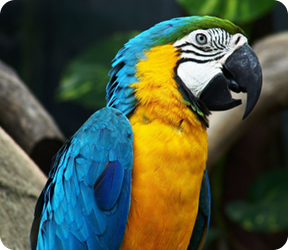
\includegraphics[scale=0.6]{figures/arara.png}
\caption{A lovely photo of an arara.}
\label{fig:arara}
\end{figure}

Lovely bird, isn't it? Now, you are probably wondering why I chose this name. Well, araras are colorful, noisy,
naughty and very funny. Everybody loves araras. So why can't you love a tool with the very same name? And
there is also another motivation of the name \emph{arara}: the chatroom residents of 
\href{http://chat.stackexchange.com/rooms/41}{\TeX.sx} -- including myself -- are fans of palindromes,
especially palindromic numbers. As you can already tell, \emph{arara} is a palindrome.

\section{How does it work?}
\label{sec:howdoesitwork}

Now that we know what \arara is, let's take a look on how the tool actually works. The whole idea is pretty
straightforward, but some concepts might be confusing at first. Do not despair, we will come back to
them later on in the manual, in Chapter~\ref{chap:importantconcepts}.

First of all, we need to add at least one instruction in the source code to tell \arara what to do. This instruction
is named \emph{directive} and it will be parsed during the preparation phase. By default, an \arara directive is
defined in a line of its own, started with a comment, followed by the word |arara:|  and the name of the task.
Code~\ref{code:hellolatex} has one directive, referencing |pdflatex|. It's important to observe that |pdflatex|
is not the command to be executed, but the name of the rule associated with that directive.

Once \arara finds a directive, it will look for the associated \emph{rule}. In our example, it will look for a rule named
|pdflatex| which will evidently run the |pdflatex|  command line application. The rule is analyzed, all possible
parameters are defined, the command line call is built and then it goes to a queue of commands to be executed.

After extracting all directives from a source code and mapping each one of them to their respective rules, \arara
then executes the queue of commands. The execution chain requires that the command $i$ was successfully
executed to then proceed to the command $i+1$, and so forth. This is also by design: \arara will halt the execution
if any of the commands in the queue had raised an error. If we run \arara on |mydoc.tex| -- we can also run
|arara mydoc| too, we will discuss this later on -- presented in Code~\ref{code:hellolatex}, we get the output
presented in Code~\ref{code:araraoutputexample}.

\begin{code}[htbp]
\caption{Running \arara on \mycmd{mydoc.tex}.}
\label{code:araraoutputexample}
\begin{bash}
$ arara mydoc
  __ _ _ __ __ _ _ __ __ _
 / _` | '__/ _` | '__/ _` |
| (_| | | | (_| | | | (_| |
 \__,_|_|  \__,_|_|  \__,_|

Running PDFLaTeX... SUCCESS
\end{bash}
\end{code}

That is pretty much how \arara works: directives in the source code are mapped to rules, which are converted to
commands and added to a queue. The queue is then executed and the status is reported. We will cover more details
about the expansion process later on in the manual. In short, we teach \arara to do a task by providing a rule,
and tell it to execute it via directives in the source code.

\section{Features}
\label{sec:features}

To name a few features I like in \arara, I'd mention the ability to write rules in a human-readable format called YAML,
which rhymes with the word \emph{camel}. YAML is actually a recursive acronym for \emph{YAML Ain't Markup Language},
and it's known as a human friendly data serialization standard for all programming languages~\cite{yaml:2001}. So far,
I think this format is quite suitable to write rules, specially if you want to avoid the need of writing complicated XML mappings or
even injecting code directly into the application.

Another feature worth mentioning is the fact that \arara is platform independent. The application was written in Java,
so \arara runs on top of a Java virtual machine, available on all the major operating systems~--~in some cases, you
might need to install the proper virtual machine. We tried very hard to keep both code and libraries compatible with
older virtual machines or from other vendors. Currently, \arara is known to run on Oracle's Java 5, 6 and 7, and OpenJDK 6 and 7.
In Chapter~\ref{chap:buildingfromsources}, there are instructions on how to build \arara from sources. Even if
you use multiple operating systems, \arara should behave the same, including the rules. There are helper functions
available in order to provide support for system-specific rules based on the underlying operating system, presented
in Section~\ref{sec:functions}.

From version 3.0 on, \arara can now display localized messages. The default language is set to English, but the user can
receive feedback from the execution process and logging in other languages as well, such as Brazilian Portuguese, German,
Italian, French, Spanish, Russian and Turkish. There's also a way to redefine the default language by adding an entry in the configuration
file, discussed later on in Section~\ref{sec:language}.

Speaking of which, \arara has now an optional configuration file in which we can add rule paths, set the default language and
define custom extensions and directive patterns, located in the user home directory. That way, we can extend \arara's behaviour
to deal with other extensions, such as |.c| files, and use the tool with other formats. We will come back on this subject later on
in Chapter~\ref{chap:configurationfile}.

\arara is also easily integrated with other \TeX\ integrated development environment, such as \TeX works~\cite{texworks:2009}, an 
environment for authoring \TeX\ documents shipped with both \TeX\ Live and MiK\TeX. Chapter~\ref{chap:ideintegration} covers
the integration of \arara with several environments.

\section{Common uses}
\label{sec:commonuses}

\arara can be used in complex workflows, like theses and books. You can tell \arara to compile the document, generate
indices and apply styles, remove temporary files, compile other |.tex| documents, create glossaries, call |pdfcrop|, move files,
run \hologo{METAPOST} or \hologo{METAFONT}, and so forth. You can easily come up with your own rules.

There's an \href{http://latex-community.org/know-how/435-gnuplot-arara}{article} available in the \LaTeX\ community which
describes the integration of |gnuplot| and \arara~\cite{cereda:2012}. This article was submitted as an entry to a contest organized
by Stefan Kottwitz. It might be worth a read.

Let's see a few examples. Code~\ref{code:exlatexone} contains the workflow I used for another article I recently wrote. Note that the first call to
|pdflatex| creates the |.aux| file, then |bibtex| will extract the cited publications. The next calls to |pdflatex| will insert
and refine the references.

\begin{code}[htbp]
\caption{\mycmd{article.tex}}
\label{code:exlatexone}
\begin{latex}
% (*@@*)arara: pdflatex
% (*@@*)arara: bibtex
% (*@@*)arara: pdflatex
% (*@@*)arara: pdflatex
\documentclass[journal]{IEEEtran}
...
\end{latex}
\end{code}

Code~\ref{code:exlatextwo} contains another workflow I used for a manual. I had to use a package that required shell escape,
so the calls to |pdflatex| had to enable it. Also, I had an index with a custom formatting, then |makeindex| was called with the
 proper style.

\begin{code}[htbp]
\caption{\mycmd{manual.tex}}
\label{code:exlatextwo}
\begin{latex}
% (*@@*)arara: pdflatex: { shell: yes }
% (*@@*)arara: makeindex: { style: mystyle }
% (*@@*)arara: pdflatex: { shell: yes }
% (*@@*)arara: pdflatex: { shell: yes }
\documentclass{book}
...
\end{latex}
\end{code}

And of course, the \arara user manual is also compiled with |arara|. You can take a look in the source code and check the
header. By the way, note that I had to use a trick to avoid |arara| to read the example directives in this manual. As we will
see later, \arara reads directives everywhere. Actually, I could have changed the directive pattern for |.tex| files through
the configuration file, but that's another story.

Other workflows can be easily created. There can be an arbitrary number of instructions for \arara to execute, so feel free to
come up with your own workflow. \arara will handle it for you. My friend Joseph Wright wrote a great article about \arara in
his personal blog, it's really worth a read~\cite{wright:2012}.

I really hope you like my humble contribution to the \TeX\ community. Let \arara enhance your \TeX\ experience, it will help you
when you'll need it the most. Enjoy the manual.

\printbibliography[heading=subbibliography]

\chapter{Installation}
\label{chap:installation}

\epigraph{\emph{Adjust \texttt{\string\hsize}: old man Fermat couldn't.}}{Enrico Gregorio}

Spledid, so you decided to give \arara a try? This chapter will cover the installation procedure. We basically
have two methods of installing \arara: the first one is through a cross-platform installer, which is of course
the recommended method; the second one is a manual deployment, with the provided |.jar| file -- a
self-contained, batteries-included executable Java archive file. If you have a recent \TeX\ Live distribution,
good news: \arara is already available in your system!

\section{Prerequisites}
\label{sec:prerequisites}

I know I've mentioned this before in Section~\ref{sec:features} and, at the risk of being repetitive, there we
go again: \arara is written in Java and thus depends on a virtual machine in the underlying operating system.
If you use a Mac or even a fairly recent Linux distribution, I have good news for you: it's mostly certain that
you already have a Java virtual machine installed.

It's very easy to check if you have a Java virtual machine installed: try running |java -version| in the terminal
(bash, command prompt, you name it) and see if you get an output similar to the one provided in
Code~\ref{code:javainstalled}.

\begin{code}[htbp]
\caption{Checking if \mycmd{java} is installed.}
\label{code:javainstalled}
\begin{bash}
$ java -version
java version "1.6.0_24"
OpenJDK Runtime Environment (IcedTea6 1.11.1)
OpenJDK Client VM (build 20.0-b12, mixed mode)
\end{bash}
\end{code}

If the output goes along the lines of |java: command not found|, I'm afraid you don't have a Java virtual
machine installed in your operating system. Since the virtual machine is a prerequisite for \arara to run,
you can install one via your favorite package manager or manually install it from the binaries available
in the official \href{http://www.java.com}{Java website}. Make sure to download the correct version for
your operating system. The installation procedure is very straightforward. If you get stuck, take a look
on the installation instructions.

It's important to mention that \arara runs also with the Java virtual machine from the OpenJDK
project~\cite{openjdk:2006}, which is already available in most of the recent Linux distributions -- actually
the output from Code~\ref{code:javainstalled} shows the OpenJDK version from my Fedora machine.
Feel free to use the virtual machine you feel most comfortable with.

Speaking of virtual machines, \arara requires at least Java 5 to run. Don't worry, it's quite easy to spot the Java
version: just look at the second digit of the version string. For example, Code~\ref{code:javainstalled} outputs |1.6.0_24|, 
which means we have Java 6 installed.

\section{Obtaining \texorpdfstring{\arara}{arara}}
\label{sec:obtainingarara}

Before proceeding, we need to choose the installation method. We have two options: the first option is the easiest one,
which installs \arara through a cross-platform installer; the second option is a manual deployment.

From version 3.0 on, \arara is also available as part of the \TeX\ Live distribution. If you have a recent \TeX\ distro,
it's almost certain that you already have \arara; make sure to select it in the |tlmgr| application.

If we opt for the installer, go to the \href{http://github.com/cereda/arara/downloads}{downloads} section of the project
 repository and download |arara-3.0-installer.jar| for all operating systems or |arara-3.0-installer.exe| for Windows.
Please note that the |.exe| version is only a wrapper which will launch |arara-3.0-installer.jar| under the hood. The 
installer also requires Java.

If we want to do things the complicated way, go to the \href{http://github.com/cereda/arara/downloads}{downloads}
section of the project repository and download the |arara.jar| file, which is a self-contained, batteries-included executable
Java archive file.

In case you want to build \arara from source, please refer to Chapter~\ref{chap:buildingfromsources} which will
cover the whole process. Thanks to Apache Maven, the build process is very easy.

\section{Using the cross-platform installer}
\label{sec:usingthecrossplatforminstaller}

After downloading |arara-3.0-installer.jar| (or its |.exe| counterpart), it's now just a matter of running it.
The installer is built with IzPack~\cite{izpack:2001}, an amazing tool for packaging applications on the Java 
platform. Of course the source is also available at the project repository. Personally, I suggest you to run the
installer in privileged mode, but you can also run it in user mode -- just keep in mind that some features might
not work, like creating symbolic links or adding the application to the system path, which inevitably requires a
privileged mode.

When running |arara-3.0-installer.jar| or its |.exe| wrapper on Windows by simply double-clicking it, the installer
will automatically run in privileged mode. A general Unix-based installation can be triggered by the command
presented in Code~\ref{code:runinstaller1}. There's also an alternative command presented in 
Code~\ref{code:runinstaller2}.

\begin{code}[htbp]
\caption{Running the installer in a Unix-based system -- method 1.}
\label{code:runinstaller1}
\begin{bash}
$ sudo java -jar arara-3.0-installer.jar
\end{bash}
\end{code}

\begin{code}[htbp]
\caption{Running the installer in a Unix-based system -- method 2.}
\label{code:runinstaller2}
\begin{bash}
$ su -c 'java -jar arara-3.0-installer.jar'
\end{bash}
\end{code}

Since Windows doesn't have a similar command to |su| or |sudo|, you need to open the command prompt as
administrator and then run the command presented in Code~\ref{code:runinstallerwin}. You can right-click
the command prompt shortcut and select the ``Run as administrator\ldots'' option.

\begin{code}[htbp]
\caption{Running the installer in the Windows command prompt as administrator.}
\label{code:runinstallerwin}
\begin{bash}
C:\> java -jar arara-3.0-installer.jar
\end{bash}
\end{code}

The installation process will begin. Hopefully, the first screen of the installer will appear, which is the
language selection (Figure~\ref{fig:instlang}). By the way, if you called the installer through the command line,
please do not close the terminal! It might end the all running processes, including our installer.

\begin{figure}[htbp]
\centering
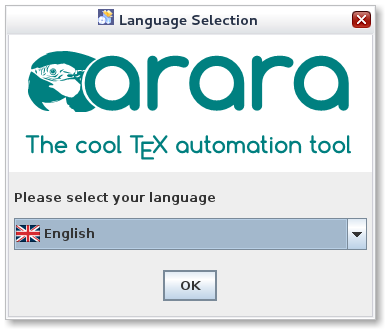
\includegraphics[scale=0.5]{figures/installer/install-langsel.png}
\caption{Language selection screen.}
\label{fig:instlang}
\end{figure}

% TODO add more languages
The installer currently supports six languages: English, German, French, Italian, Spanish, and Brazilian Portuguese.
I plan to add more languages to the list in the near feature.

The next screen welcomes you to the installation (Figure~\ref{fig:instwelcome}). There's the application name, the
current version, the team, and the project homepage. We can proceed by clicking the \textit{Next} button. 
Note that you can quit the installer at any time by clicking the \textit{Quit} button -- please, don't do it; a kitten dies
every time you abort the installation\footnote{Of course, this statement is just a joke. No animals were 
harmed, killed or severely wounded during the making of this user manual. After all, \arara is environmentally friendly.}.

\begin{figure}[htbp]
\centering
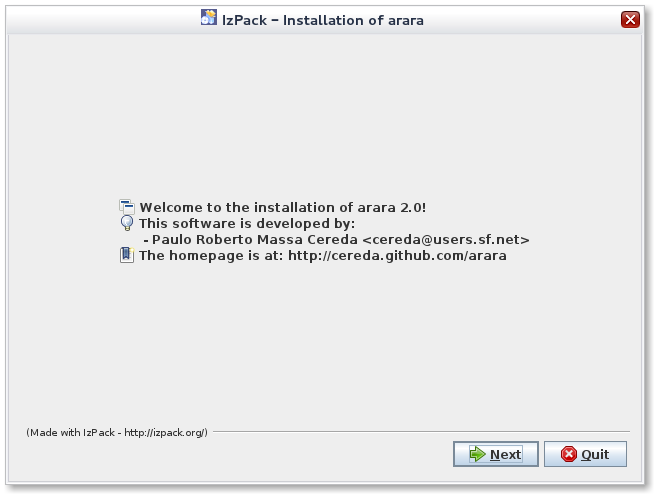
\includegraphics[scale=0.5]{figures/installer/install-welcome.png}
\caption{Welcome screen.}
\label{fig:instwelcome}
\end{figure}

Moving on, the next screen shows the license agreement (Figure~\ref{fig:instlicense}). \arara is licensed under the 
\href{http://www.opensource.org/licenses/bsd-license.php}{New BSD License}~\cite{bsd:2012}. It's important to
observe that the New BSD License has been verified as a GPL-compatible free software license by the Free Software
Foundation~\cite{fsf:1985}, and has been vetted as an open source license by the Open Source Initiative~\cite{osi:1998}.
The full license is also available in this document (page~\pageref{sec:license}). You need to accept the terms of the 
license agreement before proceeding.

The next screen is probably the most important section of the installation: in here we will choose the packs we want to
install (Figure~\ref{fig:instpacks}). All packs are described in Table~\ref{tab:packs}. Note that the grayed packs are 
required.

\begin{figure}[htbp]
\centering
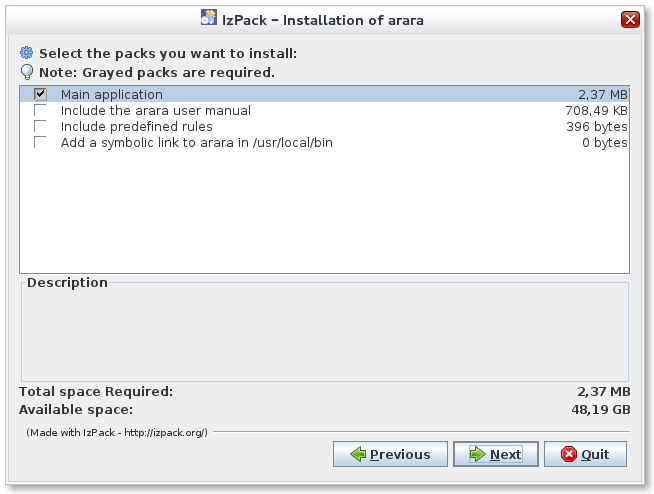
\includegraphics[scale=0.5]{figures/installer/install-packs.png}
\caption{Packs screen.}
\label{fig:instpacks}
\end{figure}

\begin{table}[htbp]
\centering
\caption{Available packs.}
\label{tab:packs}
\renewcommand{\arraystretch}{1.5}
\footnotesize
\begin{tabular}{p{0.30\textwidth}p{0.12\textwidth}p{0.4\textwidth}}
\hline
\textbf{Pack name} & \textbf{OS} & \textbf{Description}                       \\
\hline
\hline
Main application & All & This pack contains the core application. It also 
provides an |.exe| wrapper for Windows and a bash file for Unix.              \\
\hline
Include the \arara user manual & All & This pack installs this user manual into 
the |docs/| subdirectory of \arara.                                           \\
\hline
Include predefined rules & All & Of course, \arara has a set of predefined rules
for you to start with. If you prefer to write your own rules from scratch, do 
not select this pack.                                                         \\
\hline
Add a symbolic link to \arara in |/usr/local/bin| & Unix & If you ran the 
installer in privileged mode, a symbolic link to \arara can be created in the 
|/usr/local/bin| directory. There's no magic here, the installer uses the good 
old |ln| command.                                                             \\
\hline
Add \arara to the system path & Windows & Like the Unix task, \arara can also 
add itself to the system path. This feature is provided by a Windows script named
\href{http://legroom.net/software/modpath}{Modify Path}~\cite{modpath:2012}. \\
\hline
\end{tabular}
\end{table}

It's very important to mention that all these modifications in the operating 
system -- the symbolic link creation for Unix or the addition to the path for 
Windows -- are safely removed when you run the \arara uninstaller. We will talk 
about it later, in Section~\ref{sec:uninstallingarara}.

\begin{figure}[htbp]
\centering
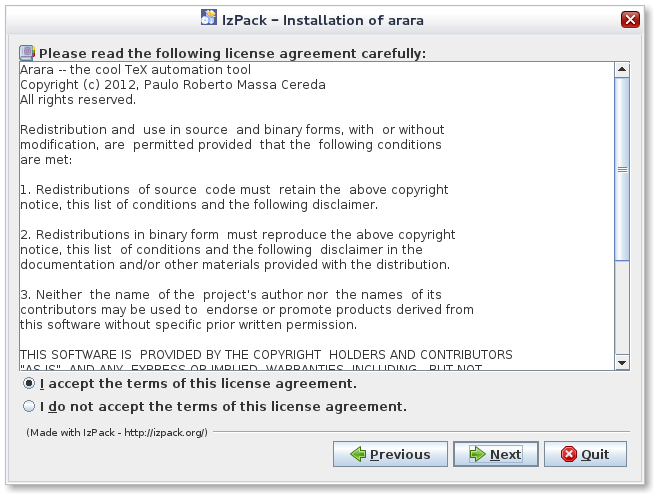
\includegraphics[scale=0.5]{figures/installer/install-license.png}
\caption{License agreement screen.}
\label{fig:instlicense}
\end{figure}

In the next screen, we will select the installation path (Figure~\ref{fig:instpath}). The installer
will automatically set the default installation path according to the Table~\ref{tab:paths}, but
feel free to install \arara in your favorite structure -- even |/opt| or your home folder.

\begin{table}[htbp]
\centering
\caption{Default installation paths.}
\label{tab:paths}
\renewcommand{\arraystretch}{1.5}
\begin{tabular}{cl}
\hline
\textbf{OS} & \textbf{Default installation path}\\
\hline
\hline
Windows & |C:\Program Files\arara|\\
Unix & |/usr/local/arara|\\
\hline
\end{tabular}
\end{table}

\begin{figure}[htbp]
\centering
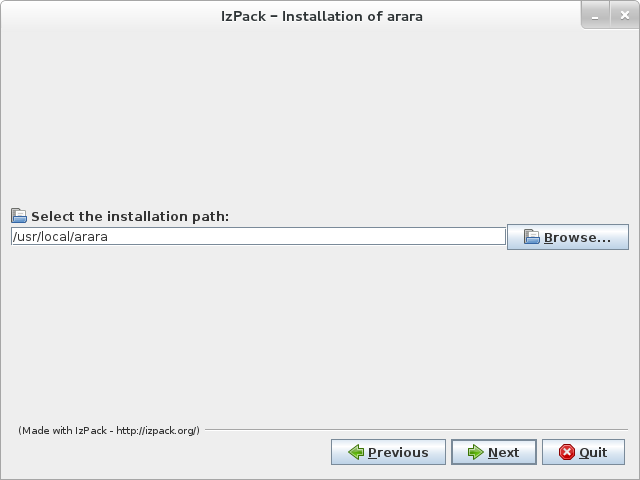
\includegraphics[scale=0.5]{figures/installer/install-path.png}
\caption{Installation path screen.}
\label{fig:instpath}
\end{figure}

After selecting the installation path, the installer will then confirm the creation of the target directory
(Figure~\ref{fig:instnewfolder}). We simply click \textit{OK} to accept it. For convenience, the full installation path 
defined in the installation path screen (Figure~\ref{fig:instpath}) will be referred as |ARARA_HOME| from now on.

\begin{figure}[htbp]
\centering
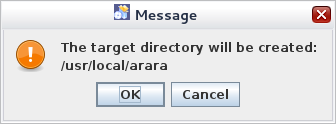
\includegraphics[scale=0.5]{figures/installer/install-pathwarning.png}
\caption{Target directory confirmation.}
\label{fig:instnewfolder}
\end{figure}

Now, just sit back and relax while \arara is being installed (Figure~\ref{fig:instprogress}). All selected packs will
be installed accordingly. The post installation tasks -- like creating the symbolic link or adding \arara to the system
path -- are performed here as well. If the installation has completed successfully, we will reach the final screen of
the installer congratulating us for installing \arara (Figure~\ref{fig:instfinish}).

\begin{figure}[htbp]
\centering
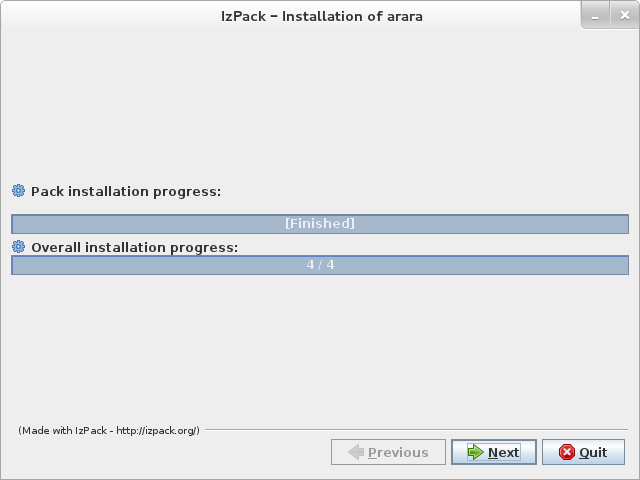
\includegraphics[scale=0.5]{figures/installer/install-progress.png}
\caption{Progress screen.}
\label{fig:instprogress}
\end{figure}

\begin{figure}[htbp]
\centering
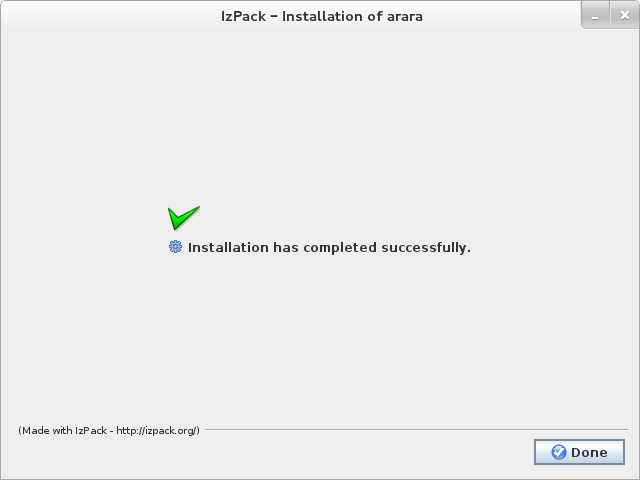
\includegraphics[scale=0.5]{figures/installer/install-finish.png}
\caption{Final screen.}
\label{fig:instfinish}
\end{figure}

The full installation scheme is presented in Figure~\ref{fig:ararastructure}. The directory structure is
presented here as a whole; keep in mind that some parts will be omitted according to your operating
system and pack selection. For example, the |etc/| subdirectory will only be installed if and only if
you are in Windows and the system path pack is selected. Other files are platform-specific, such as
|arara.exe| for Windows and the |arara| bash file for Unix.

\begin{figure}[htbp]
\centering
\begin{tikzpicture}[grow via three points={one child at (0.5,-0.7) and two children at (0.5,-0.7) and (0.5,-1.4)}, edge from parent path={(\tikzparentnode.south) |- (\tikzchildnode.west)}, anchor=west, font=\ttfamily]
  \node {ARARA\_HOME/}
    child { node {arara.jar}}		
    child { node {arara.exe}}
    child { node {arara}}
    child { node {docs/}
      child { node {arara-usermanual.pdf}}
    }
    child [missing] {}
    child { node {etc/}
      child { node {modpath.exe}}
    }
    child [missing] {}
    child { node {Uninstaller/}
      child { node {uninstaller.jar}}
    }
	child [missing] {}
	  child { node {rules/}
        child { node {biber.yaml}}
        child { node {\ldots}}
        child { node {xetex.yaml}}
    };
\end{tikzpicture}
\caption{Installation scheme.}
\label{fig:ararastructure}
\end{figure}

That's it, \arara is installed in your operating system. If you opted for the symbolic link creation or the path addition,
\arara is already available in your terminal by simply typing |arara|. Have fun!

\section{Manual installation}
\label{sec:manualinstallation}

Thankfully, \arara is also very easy to be manually deployed. First of all, we must create the application directory.
Feel free to create this directory anywhere in your computer; it can be |C:\arara|, |/opt/arara| or another location 
of your choice. This procedure is similar to the installation path screen (Figure~\ref{fig:instpath}) from
Section~\ref{sec:installer}. Again, for convenience, the full installation path will be referred as |ARARA_HOME| from 
now on. Although it's not mandatory, try to avoid folders structures with spaces in the path. In any case,
\arara can handle such spaces.

After downloading |arara.jar| from the \href{http://github.com/cereda/arara/downloads}{downloads} section of
the project repository, let's copy it to the |ARARA_HOME| directory we've created in the previous step.
Since |arara.jar| is a self-contained, batteries-included executable Java archive file, \arara is already installed.

In order to run \arara from a manual installation, we should open a terminal and run |java -jar $ARARA_HOME/arara.jar|,
but that is far from being intuitive. To make our lives easier, we will create a shortcut for this
command.

If you are deploying \arara in Windows, there are two methods for creating a shortcut: the first method -- the
easiest -- consists of downloading the |arara.exe| wrapper from the \href{http://github.com/cereda/arara/downloads}{downloads}
section and copying it to the |ARARA_HOME| directory, in the same level of |arara.jar|. This |.exe| wrapper, provided by \href{http://launch4j.sourceforge.net}{Launch4J}~\cite{launch4j:2005}, wraps |.jar| files in Windows native executables
and allows to run them like a regular Windows program.

The second method for creating a shortcut in Windows is to provide a batch file which will call |java -jar $ARARA_HOME/arara.jar|
for us. Create a file named |arara.bat| or |arara.cmd| inside the |ARARA_HOME| directory, in the same level of |arara.jar|, and
add the content from Code~\ref{code:windows}.

\begin{code}[htbp]
\caption{Creating a batch file for \arara in Windows.}
\label{code:windows}
\begin{bash}
@echo off
java -jar "%~dp0\arara.jar" %*
\end{bash}
\end{code}

After creating the batch file, add the full |ARARA_HOME| path to the system path. Unfortunately, this manual can't cover
the path settings, since it's again a matter of personal taste. I'm sure you can find tutorials on how to add a directory to
the system path.

If you are deploying \arara in Linux or Mac, we also need to create a shortcut to |java -jar $ARARA_HOME/arara.jar|.
Create a file named |arara| inside the |ARARA_HOME| directory, in the same level of |arara.jar|, and add the content 
from Code~\ref{code:unix}.

\begin{code}[htbp]
\caption{Creating a script for \arara in Linux and Mac.}
\label{code:unix}
\begin{bash}
#!/bin/bash
# Example script of arara
# Installation and usage are described in the documentation
SOURCE="${BASH_SOURCE[0]}"
while [ -h "$SOURCE" ] ; do SOURCE="$(readlink "$SOURCE")"; done
DIR="$( cd "$( dirname "${BASH_SOURCE[0]}" )" && cd -P "$( dirname "$SOURCE" )" && pwd )"
java -jar "$DIR/arara.jar" "$@"
\end{bash}
\end{code}

We now need to add execute permissions for our newly created script through |chmod +x arara|. The |arara| script can
be invoked through path addition or symbolic link. I personally prefer to add |ARARA_HOME| to my user path, but a
symbolic link creation seems way more robust -- it's what the installer does. Anyway, it's up to you to decide which method
you want to use. There's no need to use both.

Once we conclude the manual installation, it's time to check if \arara is working properly. Try running |arara| in the terminal
and see if you get the output shown in Code~\ref{code:arararun}.

\begin{code}[p]
\caption{Testing if \arara is working properly.}
\label{code:arararun}
\begin{nolanguage}
$ arara 
  __ _ _ __ __ _ _ __ __ _ 
 / _` | '__/ _` | '__/ _` |
| (_| | | | (_| | | | (_| |
 \__,_|_|  \__,_|_|  \__,_|

arara 3.0 - The cool TeX automation tool
Copyright (c) 2012, Paulo Roberto Massa Cereda
All rights reserved.

usage: arara [file [--log] [--verbose] [--timeout N] [--language L] | --help | --version]

 -h,--help             print the help message
 -L,--language <arg>   set the application language
 -l,--log              generate a log output
 -t,--timeout <arg>    set the execution timeout (in milliseconds)
 -v,--verbose          print the command output
 -V,--version          print the application version
\end{nolanguage}
\end{code}

If the terminal doesn't display the \arara logo and usage, please review the manual installation steps.
Every step is important in order to make \arara available in your system. You can also try the cross-platform
installer. If you still have any doubts, feel free to contact us.

\section{Updating \texorpdfstring{\arara}{arara}}
\label{sec:updatingarara}

If there is a newer version of \arara available in the \href{http://github.com/cereda/arara/downloads}{downloads}
section of the project repository, simply download the |arara.jar| file and copy it to the |ARARA_HOME| directory,
replacing the current one. No further steps are needed, the newer version is deployed. Try running |arara --version|
in the terminaland see if the version shown in the output is equal to the one you have downloaded.

Anyway, for every version, \arara has the proper cross-platform installer available for download in the project repository.
You can always uninstall the old \arara setup and install the new one. Please note that only major versions are released
with the installer.

If you have \arara through the \TeX\ Live distribution, the update process is straightforward: simply open a
terminal and run |tlmgr update arara| in order to update the application. This is of course the preferred method.

\section{Uninstalling \texorpdfstring{\arara}{arara}}
\label{sec:uninstallingarara}

If you want to uninstall \arara, there are two methods available. If you installed \arara through the cross-platform installer,
I have good news for you: it's just a matter of running the uninstaller. Now, if \arara was deployed through the manual
installation, we might have to remove some links or path additions.

A general Unix-based uninstallation can be triggered by the command presented in Code~\ref{code:uninstall1}.
There's also an alternative command presented in Code~\ref{code:uninstall2}.

\begin{code}[htbp]
\caption{Running the uninstaller in a Unix-based system -- method 1.}
\label{code:uninstall1}
\begin{bash}
$ sudo java -jar $ARARA_HOME/Uninstaller/uninstaller.jar
\end{bash}
\end{code}

\begin{code}[htbp]
\caption{Running the uninstaller in a Unix-based system -- method 2.}
\label{code:uninstall2}
\begin{bash}
$ su -c 'java -jar $ARARA_HOME/Uninstaller/uninstaller.jar'
\end{bash}
\end{code}

Since Windows doesn't have a similar command to |su| or |sudo|, you need to open the command prompt as administrator
and then run the command presented in Code~\ref{code:uninstallwin}. You can right-click the command prompt shortcut 
and select the ``Run as administrator\ldots'' option.

\begin{code}[htbp]
\caption{Running the uninstaller in the Windows command prompt as administrator.}
\label{code:uninstallwin}
\begin{bash}
C:\> java -jar $ARARA_HOME/Uninstaller/uninstaller.jar
\end{bash}
\end{code}

The uninstallation process will begin. Hopefully, the first and only creen of the uninstaller will appear
(Figure~\ref{fig:uninstallone}). By the way, if you called the uninstaller through the command line, please
do not close the terminal! It might end the all running processes, including our uninstaller.

\begin{figure}[htbp]
\centering
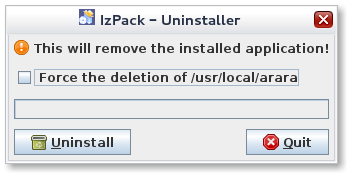
\includegraphics[scale=0.5]{figures/installer/uninstall-welcome.png}
\caption{The uninstaller screen.}
\label{fig:uninstallone}
\end{figure}

There's nothing much to see in the uninstaller. We have an option to force the deletion of the |ARARA_HOME| directory,
but that's all. By clicking the \textit{Uninstall} button, the uninstaller will remove the symbolic link or the path entry for
\arara from the operating system, if selected during the installation. Then it will erase the |ARARA_HOME| directory 
(Figure~\ref{fig:uninstalltwo}).

\begin{figure}[htbp]
\centering
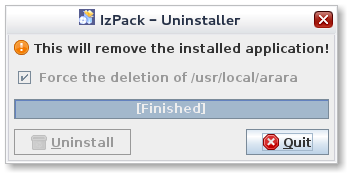
\includegraphics[scale=0.5]{figures/installer/uninstall-finish.png}
\caption{The uninstaller screen, after the execution.}
\label{fig:uninstalltwo}
\end{figure}

Unfortunately, even if you force the deletion of the |ARARA_HOME| directory in Windows, the operating system can't
remove the |Uninstaller| subdirectory because the uninstaller was being executed from there. But that's the only trace 
left. You can safely delete |ARARA_HOME| after running the uninstaller.

If \arara was manually installed, we need to remove the symbolic link reference or the path entry, if any, then delete
the |ARARA_HOME| directory. Don't leave any traces of \arara in system directories or configuration files; a broken 
symbolic link or a wrong path entry might cause trouble in the future.

\printbibliography[heading=subbibliography]

\chapter{Building from sources}
\label{chap:buildingfromsources}

\epigraph{\emph{Knowledge brings fear.}}{From a \emph{Futurama} episode}

Although \arara already features a self-contained, batteries-included executable Java archive file, an |.exe| wrapper, and a cross-platform
installer, you can easily build it from sources. The only requirements are a working Java Development Kit~\cite{oracle:2012}
and the Apache Maven software project management~\cite{maven:2012}. The next sections will cover the entire process, 
from obtaining the sources to the build itself. Sadly, this manual doesn't cover Java and Maven deployments, so I kindly ask you
to check their websites and read the available documentation.

\section{Obtaining the sources}
\label{sec:obtainingthesources}

First of all, we need to get the source code, available in the project repository hosted on \href{https://github.com/cereda/arara}{GitHub}.
We have two options on how to obtain the sources: either by clicking the \href{https://github.com/cereda/arara/archive/master.zip}{Zip} button in the project page and download a snapshot
of the whole structure in an archive file, or by using |git| and clone the repository into our machine. The second option is easily done by executing the command presented in Code~\ref{code:gitobtain}, provided of course that you have |git|  installed.

\begin{code}[htbp]
\caption{Cloning the project repository.}
\label{code:gitobtain}
\begin{bash}
$ git clone git://github.com/cereda/arara.git
\end{bash}
\end{code}

After cloning the project repository (Code~\ref{code:gitobtain}), a new subdirectory named |arara| is created in the current directory
with the project structure -- the very same available in the project repository on GitHub. The application source code is inside
|arara/arara|. Note that there are other source codes for the cross-platform installer and the |.exe| wrapper, as well as the predefined
rules, each one in a subdirectory of its own.

If you opted for downloading the archive file, you'll have a file named |arara-master.zip| generated automatically by GitHub.
Just extract the file somewhere in your computer and you'll end up with the very same project structure as the one available in the
project repository.

\section{Building \texorpdfstring{\arara}{arara}}
\label{sec:buildingarara}

Inside the |arara/arara| directory, we have the most important file for building \arara: a file named |pom.xml|. We now just need to
call the |mvn| command with the proper target and relax while Maven takes care of the building process for us. First of all, let's take
a look at some targets available in our |pom.xml| file: 

\begin{ruleoptions}
\item[compile] This target compiles the source code, generating the Java bytecode.
\item[package] The |package| target is very similar to the |compile| one, but instead of only compiling the source code, it also
packs the Java bytecode into an executable Java archive file without dependencies. The file will be available inside the
|arara/arara/target| directory.
\item[assembly:assembly] This target is almost identical to the |package| one, but it also includes all the dependencies into a
final Java archive file. The file will be available inside the |arara/arara/target| directory. This is of course our preferred target,
since \arara is shipped as a self-contained executable Java archive file.
\item[clean] The |clean| target removes all the generated Java bytecode and deployment traces, cleaning the project structure.
\end{ruleoptions}

Now that we know the targets, we only need to call |mvn| with the target we want. If you want to generate the very same Java archive file
we use for releases, execute the command presented in Code~\ref{code:mvnassembly}.

\begin{code}[htbp]
\caption{Building \arara with Maven, first attempt.}
\label{code:mvnassembly}
\begin{bash}
$ mvn assembly:assembly
\end{bash}
\end{code}

Actually, the command presented in Code~\ref{code:mvnassembly}, as the project structure is at the moment, will fail! Let me explain
why: the application is not yet linked with the localized messages, so we need to convert our translation files into a correct format and
then run the target in Maven. The error message after running |mvn assembly:assembly| presented in Code~\ref{code:errorlangnotfound}
gives us a hint on what we should do.

\begin{code}[htbp]
\caption{The Maven error message about missing localization files.}
\label{code:errorlangnotfound}
\begin{bash}
Failed tests: testLocalizationFile(com.github.arara.AraraTest):
arara requires at least the default localization file
Messages.properties located at the translations/ directory in
the project repository. Rename Messages.input to
Messages.properties and copy the new file to the src/
directory, under com/github/arara/localization, and build
arara again.

Tests run: 1, Failures: 1, Errors: 0, Skipped: 0

[INFO] ---------------------------------------------
[INFO] BUILD FAILURE
[INFO] ---------------------------------------------
\end{bash}
\end{code}

Let's go into |arara/translations| and run the commands presented in Code~\ref{code:convertinglocales}. Since we are dealing with
languages that require an encoding in UTF-8 while the localization files are set in ASCII, we need to run a conversion program in
order to generate valid |.properties|  files.

\begin{code}[htbp]
\caption{Converting the localization files.}
\label{code:convertinglocales}
\begin{bash}
$ native2ascii -encoding utf8 Messages.input ../application/src/main/resources/com/github/arara/localization/Messages.properties
$ native2ascii -encoding utf8 Messages_de.input ../application/src/main/resources/com/github/arara/localization/Messages_de.properties
$ native2ascii -encoding utf8 Messages_es.input ../application/src/main/resources/com/github/arara/localization/Messages_es.properties
$ native2ascii -encoding utf8 Messages_fr.input ../application/src/main/resources/com/github/arara/localization/Messages_fr.properties
$ native2ascii -encoding utf8 Messages_it.input ../application/src/main/resources/com/github/arara/localization/Messages_it.properties
$ native2ascii -encoding utf8 Messages_pt_BR.input ../application/src/main/resources/com/github/arara/localization/Messages_pt_BR.properties
$ native2ascii -encoding utf8 Messages_ru.input ../application/src/main/resources/com/github/arara/localization/Messages_ru.properties
$ native2ascii -encoding utf8 Messages_tr.input ../application/src/main/resources/com/github/arara/localization/Messages_tr.properties
\end{bash}
\end{code}

Now we can simply rerun the command presented in Code~\ref{code:mvnassembly}. Hopefully, we won't have trouble this time.
Relax while Maven takes care of the building process. It might take a while, since all dependencies will be downloaded to your Maven repository. After a while, Maven will tell us that the project was built successfully!

After a successful build via Maven, we can now get the generated executable Java archive file |arara-3.0-with-dependencies.jar| which is inside the |arara/arara/target| directory, rename it to |arara.jar| and use it as we have seen in the previous chapters.

\section{Notes on the installer and wrapper}
\label{sec:notesontheinstallerandwrapper}

The project directory has additional subdirectories regarding the \arara cross-platform installer and the |.exe| wrapper. It's important to
observe that only the build files are available, which means that you need to review the compilation process and make adjustments
according to your directory structure. 

The cross-platform installer Java archive file is generated with IzPack~\cite{izpack:2001}, while the |.exe| wrapper is built with
Launch4J~\cite{launch4j:2005}. Both build files are written in plain XML, so you can easily adapt them to your needs. Sadly, the main
purpose of this chapter is to cover the build process of \arara itself and not its helper tools; if you want to generate your own wrapper
or installer, please refer to the available documentation on how to build each file. The build process is also very straightforward.

\printbibliography[heading=subbibliography]

\chapter{IDE integration}
\label{chap:ideintegration}

\epigraph{\emph{The answer to ``can Emacs\ldots'' is always ``yes''.}}{David Carlisle}

This chapter covers the integration of \arara with several integrated development environments. For obvious reasons, it's almost
impossible for us to cover the full range of editors available nowadays, so we tried to focus only on a couple of them. If you use
\arara with an IDE other than the ones listed here, please let us know! It would be great to include your contribution in this user
manual.

\section{\texorpdfstring{\TeX works}{TeXworks}}
\label{sex:texworks}

\arara can be easily integrated with \TeX works~\cite{texworks:2009}, an environment for authoring \TeX\ documents shipped
with both \TeX\ Live and MiK\TeX. In this section, we will learn how to integrate \arara and this cross-platform \TeX\ front-end
program.

First of all, make sure \arara is properly installed in your operating system. Thankfully, it's very easy to add a new tool in \TeX works,
just open the program and click in \textit{Edit} $\rightarrow$ \textit{Preferences\ldots} to open the preferences screen (Figure~\ref{fig:texworkspref}).

\begin{figure}[htbp]
\centering
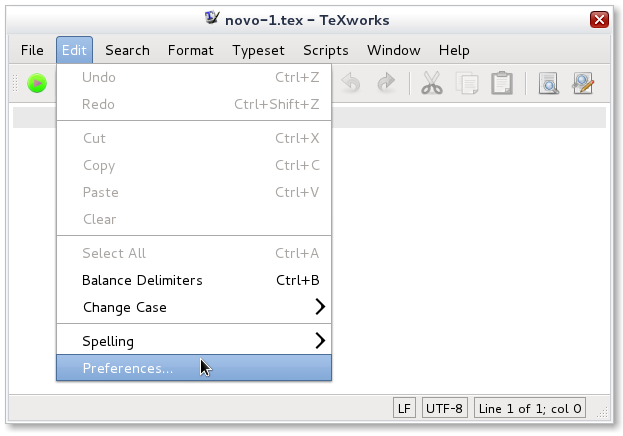
\includegraphics[scale=0.5]{figures/texworks/texworks-prefs.png}
\caption{Opening the preferences screen in \TeX works.}
\label{fig:texworkspref}
\end{figure}

The next screen is the \TeX works preferences (Figure~\ref{fig:texworksprefscreen}). There are several tabs available. Navigate to the
\textit{Typesetting} tab, which contains two lists: the paths for \TeX\ and related programs, and the processing tools. In the second
list -- the processing tools -- click the \textit{Plus (+)} button to add another tool.

\begin{figure}[htbp]
\centering
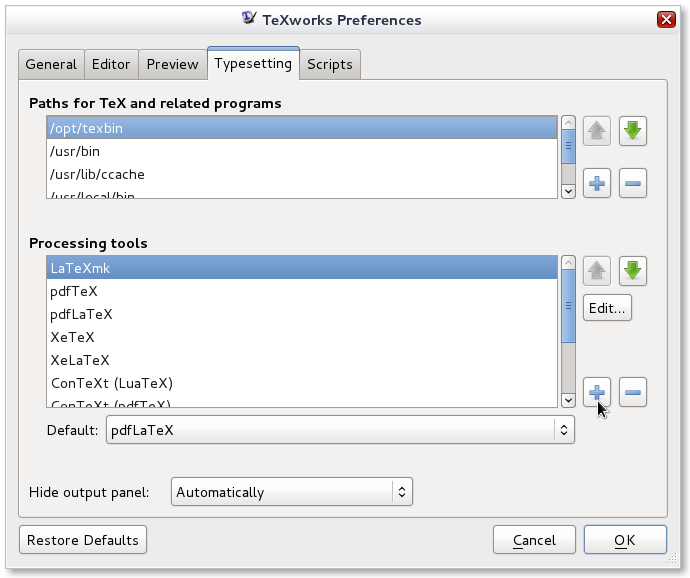
\includegraphics[scale=0.5]{figures/texworks/texworks-add.png}
\caption{The \TeX works preferences screen.}
\label{fig:texworksprefscreen}
\end{figure}

We are now in the new tool screen (Figure~\ref{fig:texworksarara}). \TeX works provides an very straightforward interface for adding
new tools; we just need to provide the tool name, the executable path, and the parameters. Table~\ref{tab:texworksarara} helps us on
what to type in each field. When done, just click \textit{OK} and our new tool will be available.

\begin{figure}[htbp]
\centering
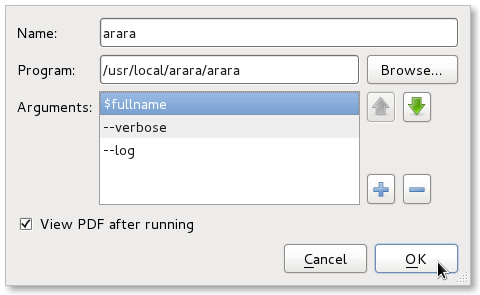
\includegraphics[scale=0.5]{figures/texworks/texworks-arara.png}
\caption{The new tool screen.}
\label{fig:texworksarara}
\end{figure}

{\renewcommand{\arraystretch}{1.5}
\begin{table}[htbp]
\centering
\footnotesize
\begin{tabular}{p{0.15\textwidth}p{0.25\textwidth}p{0.50\textwidth}}
\hline
\textbf{Field name} & \textbf{Value} & \textbf{Description}                   \\
\hline
\hline
Name & |arara| & The tool name. You can actually type whatever name your heart 
desires. This value will be displayed in the compilation profile.             \\
\hline
Program & |$ARARA_HOME/arara| & The full executable path. Just browse the 
filesystem and select the correct \arara path. Observe that symbolic links are 
resolved to their full targets. For Windows, select the |.exe| wrapper; for 
Unix, select the bash script.                                                 \\
\hline
Arguments & {\renewcommand{\arraystretch}{1}
\begin{tabular}[t]{l}
|$fullname|\\
|--verbose|\\
|--log|
\end{tabular}} & The tool arguments. Note that you need to type one argument at 
a time, by clicking the \textit{Plus (+)} button. The first argument is a 
\TeX works variable which will expand to the current filename. The second and
third arguments are \arara flags, discussed later, in 
Chapter~\ref{chap:runningarara}.                                            \\
\hline
\end{tabular}
\caption{Configuring \arara in \TeX works.}
\label{tab:texworksarara}
\end{table}}

We are now back to the preferences screen (Figure~\ref{fig:texworksprefscreen}). Hopefully, \arara is in the list of processing tools.
Just click \textit{OK} to confirm the new addition. Congratulations, now \arara is available as a compilation profile in \TeX works
(Figure~\ref{fig:texworksprofile}).

\begin{figure}[htbp]
\centering
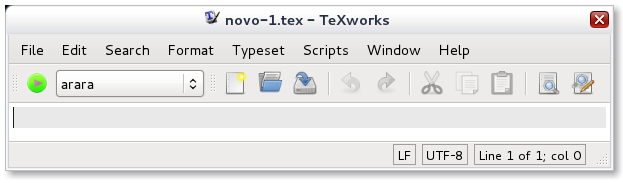
\includegraphics[scale=0.5]{figures/texworks/texworks-profile.png}
\caption{Using \arara in the \TeX works compilation profile.}
\label{fig:texworksprofile}
\end{figure}

And we are done, \arara is now integrated with \TeX works! Just make sure to select the correct profile when running the compilation
process.

\section{WinEdt}
\label{sec:winedt}

The following procedure is kindly provided by Harish Kumar. It's very easy to integrate \arara with WinEdt, let's take a look at the steps.

\subsection{Getting images for icons and toolbar}

WinEdt uses $16 \times 16$ |.png| images for menu items, the toolbar and the tree control. They are available in \texttt{\%B\textbackslash Bitmaps\textbackslash Images}\footnote{\texttt{\%B} maps to \texttt{C:\textbackslash Program Files\textbackslash WinEdt Team\textbackslash WinEdt 7} for default installation.} folder and they are automatically loaded on startup or later through the \textit{Options Interface} (or |ReloadImages| macro function). Restricted users can place additional images in their \texttt{\%b\textbackslash Bitmaps\textbackslash Images}\footnote{\texttt{\%b} maps to \texttt{C:\textbackslash Users\textbackslash <username>\textbackslash AppData\textbackslash Roaming\textbackslash WinEdt Team\textbackslash WinEdt 7} for default installation} folder. At the moment all images have a $16\times16$ dimension and use 32-bit transparent |.png| format.

The images for the \arara toolbar can be downloaded from the \href{http://github.com/cereda/arara/downloads}{downloads area} of the project repository. It would suffice to have a $16 \times 16$ |.png| image for WinEdt v7 while for WinEdt v6, one has to use $16 \times 16$ |.bmp| image. The downloaded images must be copied to \texttt{\%B\textbackslash Bitmaps\textbackslash Images} or \texttt{\%b\textbackslash Bitmaps\textbackslash Images} (depending upon the admin privileges). Once copied, WinEdt has to be restarted to load the images. Now the images should be available for use.

\subsection{Adding a menu entry}

The following steps describe how to add a menu entry for \arara in WinEdt v6 and v7.

\begin{enumerate}
\item Go to \textit{Options $\rightarrow$ Options Interface}. A side window will appear on the left side as shown in Figure~\ref{fig:optionsinterface}.
\item From the \textit{Menus and Toolbar} drop down list, select \textit{Main Menu} and double click to open the file |Main Menu.ini|.
\item In the |Main Menu.ini| file, type the code presented in Code~\ref{code:mainmenuwinedt} somewhere in the file.
\item Save the file. Now the current script has to be loaded by clicking the \textit{Load current script} button, which is the first button in the tool bar in \textit{Options Interface} window shown in Figure~\ref{fig:optionsinterface}.
\item Now in the WinEdt \textit{\TeX} menu, a submenu called \textit{Arara} should be visible and functional (Figure~\ref{fig:winedtmenu}).
\item From the \textit{Menus and Toolbar} drop down list, select \textit{Toolbar} and double click to open the file |Toolbar.ini|.
\item In the |Toolbar.ini| file, type the following line, somewhere in the file: |BUTTON="arara"|.
\item Save the file |Toolbar.ini|. Now the current script has to be loaded by clicking the \textit{Load current script} button, which is the first button in the tool bar in \textit{Options Interface} window (Figure~\ref{fig:optionsinterface}).
\item Now a button for \arara should be visible as shown in Figure~\ref{fig:wineditararabutton}.
\end{enumerate}

\begin{figure}[htbp]
\centering
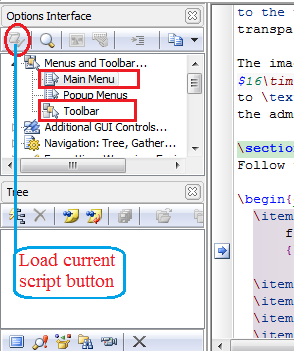
\includegraphics[width=.4\textwidth]{figures/winedt/winedt-optionsinterface.png}
\caption{The \textit{Options Interface} window in WinEdt.}
\label{fig:optionsinterface}
\end{figure}

\begin{code}[htbp]
\caption{Adding an entry to \arara in \mycmd{Main Menu.ini}.}
\label{code:mainmenuwinedt}
\begin{lstlisting}[basicstyle=\footnotesize\ttfamily, columns=flexible, showspaces=false, breaklines=true]
ITEM="Arara"
CAPTION="Arara"
IMAGE="arara16"
SAVE_INPUT=1
MACRO=:RunConsole('arara "\%F"','\%P','arara...');
REQ_FILTER=:"\%!M=TeX"|"\%!M=TeX:STY"|"\%!M=TeX:AUX"
\end{lstlisting}
\end{code}

\begin{figure}[htbp]
\centering
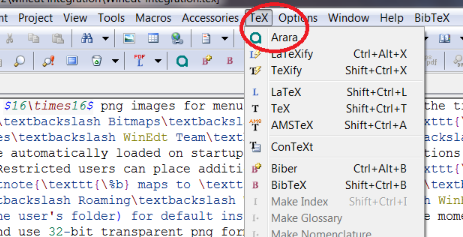
\includegraphics[width=.7\textwidth]{figures/winedt/winedt-menu.png}
\caption{The WinEdt \textit{\TeX} menu.}
\label{fig:winedtmenu}
\end{figure}

\begin{figure}[htbp]
\centering
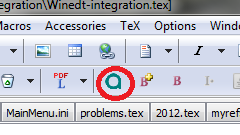
\includegraphics[width=.5\textwidth]{figures/winedt/winedt-ararabutton.png}
\caption{The \arara button in WinEdt.}
\label{fig:wineditararabutton}
\end{figure}

And we are done! \arara is successfully integrated in WinEdt. Now you can add directives to your files and click the buttons to trigger the execution.

\section{Inlage}
\label{sec:inlage}

The following procedure is kindly provided by Harish Kumar. It's very easy to integrate \arara with Inlage, let's take a look at the steps.

\subsection{Inlage v4}

The following steps describe how to add a menu entry for \arara in Inlage v4. It's an easy procedure.

\begin{enumerate}
\item Go to \textit{Build $\rightarrow$ User Commands}. A window named \textit{Edit Commands} will appear as shown in Figure~\ref{fig:inlageeditcommands}.
\item Now press the \textit{Plus (+)} button to get the \textit{Add Command} window as shown in Figure~\ref{fig:inlageaddcommand}.
\item Under the \textit{Name} textfield, type |arara| and under the \textit{Command Line} textarea, type |arara \%f|. Now the new configuration should be saved using the \textit{Save} button. Now an entry for \arara should be visible as seen in Figure~\ref{fig:inlagelistarara}.
\item These settings must be then updated using the \textit{Update} button in the \textit{Edit Commands} window shown in Figure~\ref{fig:inlageeditcommands}.
\item Now a menu entry for \arara should be visible in \textit{Build $\rightarrow$ Execute $\rightarrow$ arara}.
\end{enumerate}

\begin{figure}[htbp]
\centering
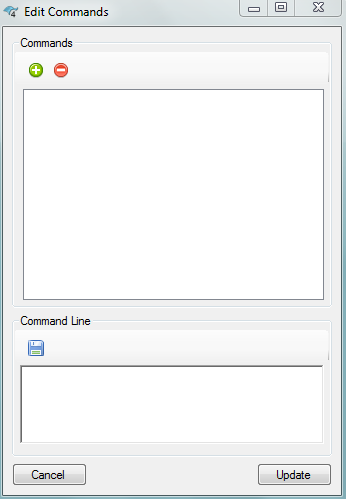
\includegraphics[width=.4\textwidth]{figures/inlage/inlage-editcommands.png}
\caption{The \textit{Edit Commands} window in Inlage.}
\label{fig:inlageeditcommands}
\end{figure}

\begin{figure}[htbp]
\centering
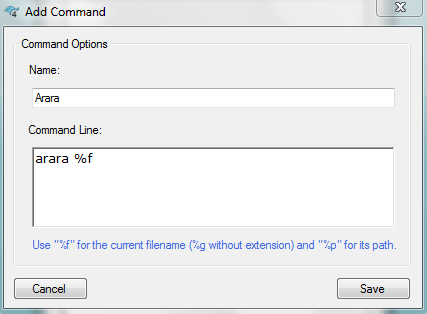
\includegraphics[width=.5\textwidth]{figures/inlage/inlage-addcommand.png}
\caption{The \textit{Add Command} window in Inlage.}
\label{fig:inlageaddcommand}
\end{figure}

\begin{figure}[htbp]
\centering
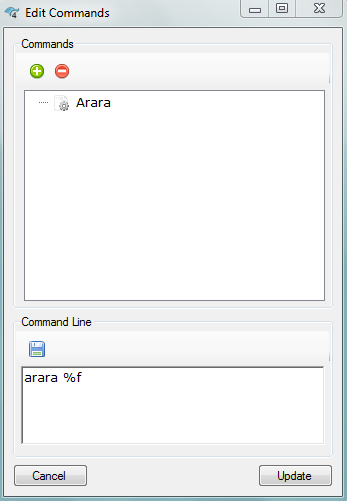
\includegraphics[width=.4\textwidth]{figures/inlage/inlage-listarara.png}
\caption{\arara added to the \textit{Edit Commands} window in Inlage.}
\label{fig:inlagelistarara}
\end{figure}

That's it, \arara is now successfully integrated in Inlage v4. Have fun!

\subsection{Inlage v5}

The following steps describe how to add a menu entry for \arara in Inlage v5. It's an easy procedure.

\begin{enumerate}
\item Go to \textit{Build $\rightarrow$ Compiler Options\ldots}. A \textit{Settings} window will appear as shown in Figure~\ref{fig:inlagesettings}.
\item Under \textit{Profiles}, create a new profile clicking the \textit{New} button. A new window will open; now let's type the name for the new profile as |arara|, as shown in Figure~\ref{fig:inlagenewprofile}. Now press \textit{Okay}.
\item Under \textit{Compiler Order}, press \textit{Add Compiler}, as shown in Figure~\ref{fig:inlageaddcompiler}.
\item Under \textit{Binaries}, change the following:
\begin{enumerate}
\item In \textit{Implementation}, choose \textit{Custom}.
\item In \textit{Binary Name}, choose the executable for \arara using the \textit{Browse} button.
\item In \textit{Parameters}, you can choose the parameters, such as |--verbose|.
\item In \textit{Target File}, choose \textit{Active File/Masterfile}.
\end{enumerate}
\item Save these settings. After the previous steps, you should get a menu for \arara in Inlage v5 as seen in Figure~\ref{fig:inlageararamenu}.
\end{enumerate}

\begin{figure}[htbp]
\centering
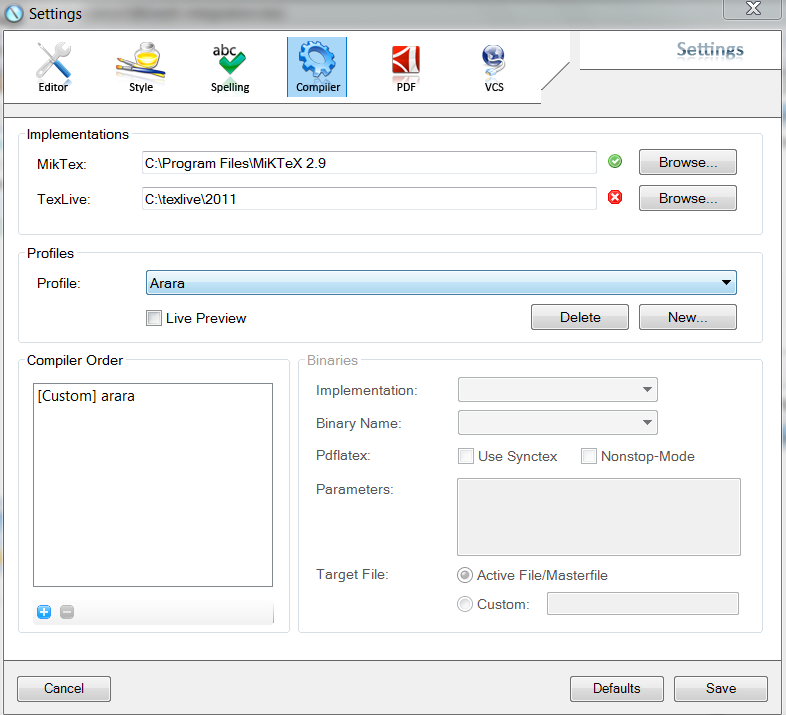
\includegraphics[width=.7\textwidth]{figures/inlage/inlage-settings.png}
\caption{The \textit{Settings} window in Inlage.}
\label{fig:inlagesettings}
\end{figure}

\begin{figure}[htbp]
\centering
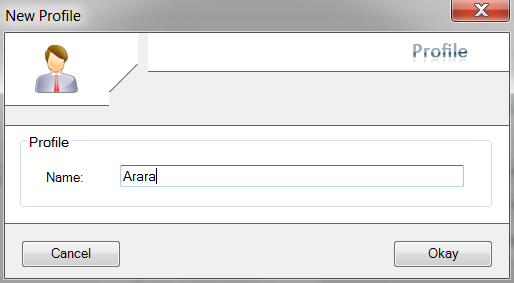
\includegraphics[width=.7\textwidth]{figures/inlage/inlage-newprofile.png}
\caption{Adding a new profile in Inlage.}
\label{fig:inlagenewprofile}
\end{figure}

\begin{figure}[htbp]
\centering
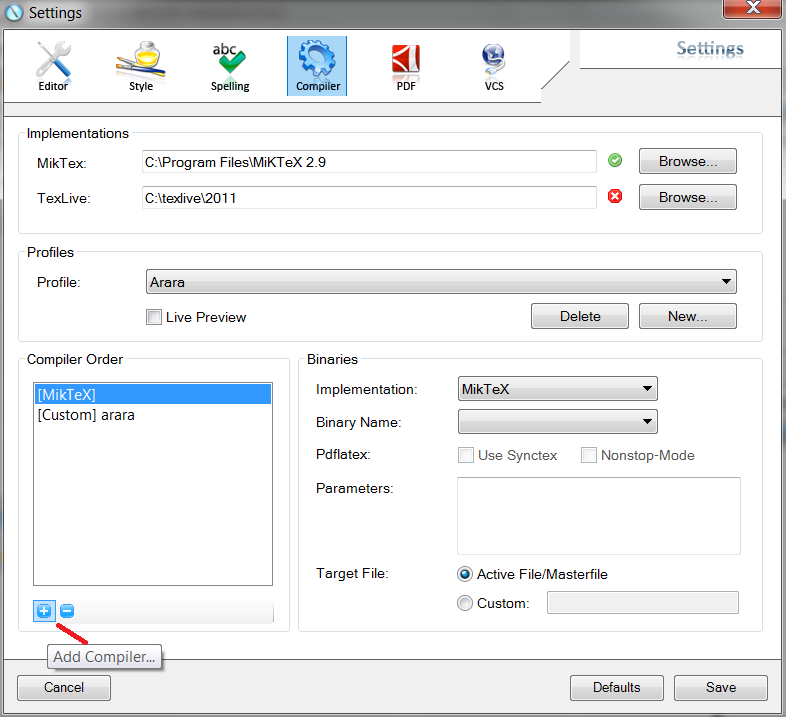
\includegraphics[width=.7\textwidth]{figures/inlage/inlage-addcompiler.png}
\caption{Adding a compiler in Inlage.}
\label{fig:inlageaddcompiler}
\end{figure}

\begin{figure}[htbp]
\centering
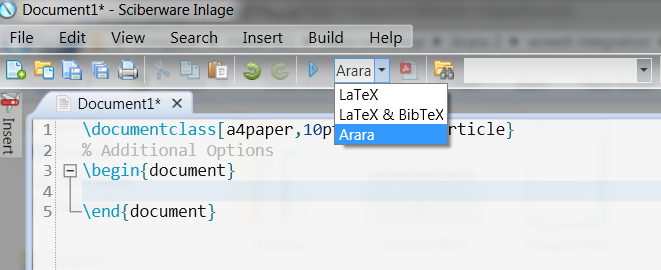
\includegraphics[width=.7\textwidth]{figures/inlage/inlage-araramenu.png}
\caption{\arara added to the menu in Inlage.}
\label{fig:inlageararamenu}
\end{figure}

That's it, \arara is successfully integrated with Inlage v5. Have fun!

\section{\texorpdfstring{\TeX Shop}{TeXShop}}
\label{sec:texshop}

Integrating \arara with \TeX shop is probably one of the easiest procedures. Simply open your terminal, go to |~/Library/TeXShop/Engines| and create a file named |arara.engine| with the content presented in Code~\ref{code:texshopcode}.

Now, we need to add execute permissions to our newly created file. A simple |chmod +x arara.engine| will do the trick. Now, open \TeX shop and you will see \arara available for use in the list of engines (Figure~\ref{fig:texshop}).

\begin{figure}[htbp]
\centering
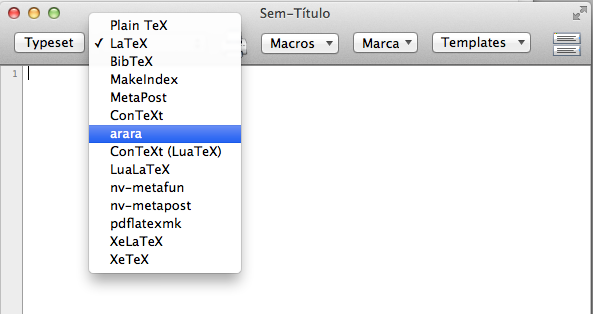
\includegraphics[width=.8\textwidth]{figures/texshop/texshop-arara.png}
\caption{\arara available in \TeX shop.}
\label{fig:texshop}
\end{figure}

No more steps are needed, \arara is successfully deployed in \TeX shop. If you want to remove \arara from \TeX shop, just remove |arara.engine| from the |Engines| directory.

\begin{code}[htbp]
\caption{\mycmd{arara.engine}}
\label{code:texshopcode}
\begin{bash}
#!/bin/bash
export PATH=/usr/texbin:/usr/local/bin:${PATH}
arara "$1"
\end{bash}
\end{code}

\section{\texorpdfstring{\TeX nic Center}{TeXnic Center}}
\label{sec:texniccenter}

\TeX nic Center has also an easy integration with \arara. The first step is to go to \textit{Build $\rightarrow$ Define Output Profiles\ldots}. The \textit{Profiles} window should open, as shown in Figure~\ref{fig:txnprofiles}.

\begin{figure}[htbp]
\centering
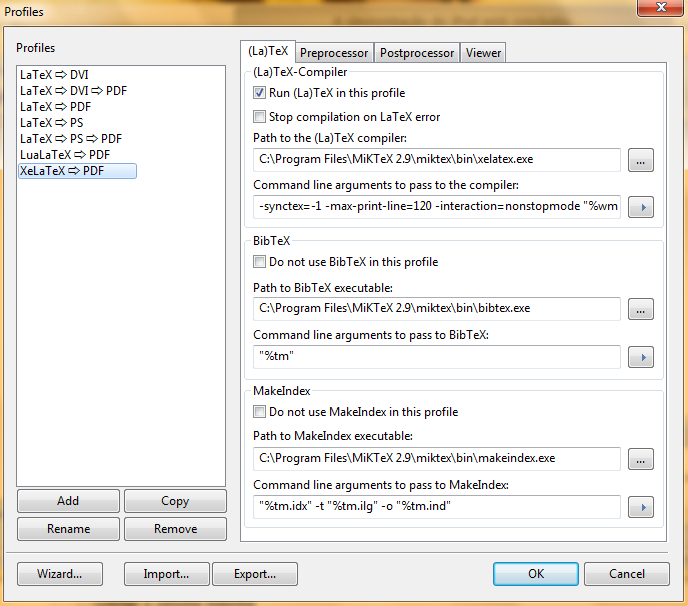
\includegraphics[width=.8\textwidth]{figures/texniccenter/texniccenter-profiles.png}
\caption{The \textit{Profiles} window in \TeX nic Center.}
\label{fig:txnprofiles}
\end{figure}

Let's now create a new profile! Click the \textit{Add} button. A window will pop up and ask for the new profile name (Figure~\ref{fig:txnnewprofile}). Type |arara| as the profile name and click \textit{OK}.

\begin{figure}[htbp]
\centering
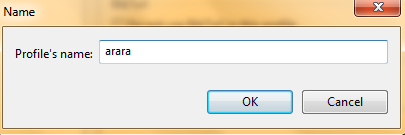
\includegraphics[width=.7\textwidth]{figures/texniccenter/texniccenter-newprofile.png}
\caption{Creating a new profile in \TeX nic Center.}
\label{fig:txnnewprofile}
\end{figure}

The last step is the easiest one. With the |arara| profile selected, check the box which says \textit{Run (La)\TeX in this profile}, then enter the full path to |arara| in the textbox named \textit{Path to the (La)\TeX compiler} and write |--log --verbose "%wm"| in the texbox named \textit{Command line arguments to pass to the compiler}; click \textit{OK}, as shown in Figure~\ref{fig:txnsettings}.

\begin{figure}[htbp]
\centering
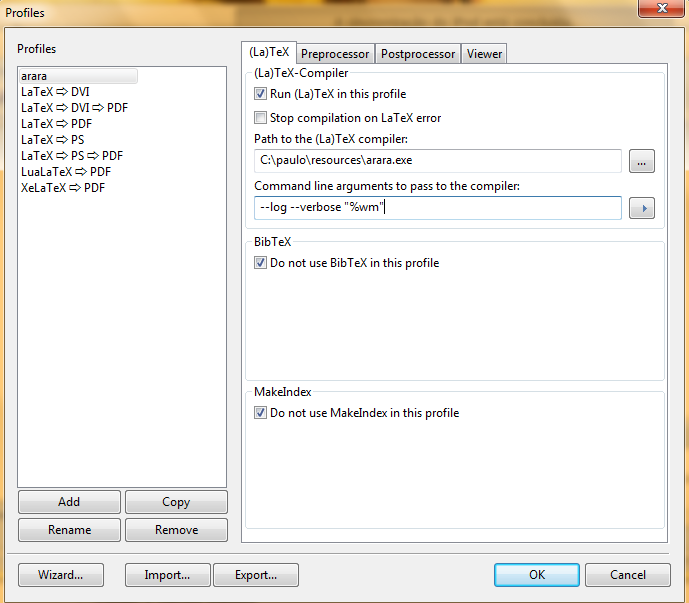
\includegraphics[width=.8\textwidth]{figures/texniccenter/texniccenter-config.png}
\caption{Configuring \arara in \TeX nic Center.}
\label{fig:txnsettings}
\end{figure}

That's it, now \arara is integrated with \TeX nic Center! Just make sure to select |arara| in the dropdown list of available profiles.

\printbibliography[heading=subbibliography]

\chapter{Important concepts}
\label{chap:importantconcepts}

\epigraph{\emph{Beware of bugs in the above code; I have only proved it correct, not tried it.}}{Donald Knuth}

Time for our first contact with \arara! It's important to understand a few concepts in which \arara relies before we proceed
to the usage itself. Do not worry, these concepts are easy to follow, yet they are vital to the comprehension of the application
and the logic behind it.

\section{Rules}
\label{sec:rules}

Do you remember |mydoc.tex| from Code~\ref{code:hellolatex} in page~\pageref{code:hellolatex}? When we tried to mimic |rubber| and
run |arara mydoc|, nothing happened. We should tell \arara how it should handle this execution. Let's start with the rules.

A \emph{rule} is a formal description of how \arara should handle a certain task. For example, if we want to use |pdflatex| with
\arara, we should have a rule for that. Once a rule is defined, \arara automatically provides an access layer to that rule through
directives, a concept to be introduced in Section~\ref{sec:directives}.

A rule is a plain text file written in the YAML format~\cite{yaml:2001}. I opted for this format because it's cleaner and more intuitive to
use than other markup languages, besides of course being a data serialization standard for all programming languages. As a bonus, the
acronym \emph{YAML} rhymes with the word \emph{camel}, so \arara is heavily environmentally friendly\footnote{Perl, I'm looking at you.}.

The default rules, that is, the rules shipped with \arara, are placed inside a special subdirectory named |rules/| inside |ARARA_HOME|. We will learn in
Section~\ref{sec:searchpaths} that we can add an arbitrary number of paths for storing our own rules, in order of priority, so don't worry
with the location of the default rules, although it's important to understand and acknowledge their existance.  The basic structure of an
\arara rule is presented in Code~\ref{code:yamlrule}.

\begin{code}[htbp]
\caption{\mycmd{makefoo.yaml}, a basic structure of an \arara rule.}
\label{code:yamlrule}
\begin{yaml}
!config
# I am a comment
identifier: makefoo
name: MakeFoo
command: makefoo @{file}
arguments: []
\end{yaml}
\end{code}

The |!config| keyword (line 1) is mandatory and it must be the first line of any \arara rule. Note that the format also accepts
comments (line 2) by simply starting a line with the |#| symbol. The following keys are defined:

\begin{ruleoptions}
\item[identifier] This key (line 3) acts as a unique identifier for the rule. It's highly recommended to use lowercase letters without
spaces, accents or punctuation symbols. As a convention, if you have an identifier named |makefoo|, the rule filename must
be |makefoo.yaml|.
\item[name] The |name| key (line 4) holds the name of the task. When running \arara, this value will be displayed in the output.
In our example, \arara will display |Running MakeFoo| in the output when dealing with this task.
\item[command] This key (line 5) contains the system command to be executed. You can use virtually any type of command,
interactive or noninteractive. But beware: if \arara is running in silent mode, which is the default behaviour, an 
interactive command wich might require the user input will be halted and the execution will fail. Don't despair, you can use a
special |--verbose| flag with \arara in order to interact with such commands -- we will talk about flags in 
Chapter~\ref{chap:runningarara}. There are cases in which you might want to have a list of commands instead of a single one;
\arara has support for multiple commands inside one rule, we just need to replace |command| by |commands|  and provide
a list of commands to be executed, as seen in Code~\ref{code:excommands}.
You probably noticed a strange element |@{file}| in the |command| line: this element is called \emph{orb tag}. For now, just admit these elements exist. We will come back to them later on, in Section~\ref{sec:orbtags}, I promise.
\item[arguments] The |arguments| key (line 6) denotes a list of arguments for the rule command. In our example, we have an empty list,
denoted as |[]|. You can define as many arguments as your command requires. Please check Code~\ref{code:makebar} for an example of a list of arguments.
\end{ruleoptions}

There are cases in which we need to run more than just one command for a certain rule. Take, for example, the |frontespizio| rule
released with \arara: when using the |frontespizio|  package\footnote{\url{http://ctan.org/pkg/frontespizio}, written by Enrico Gregorio.},
the document has to processed by the choosen engine, say |pdflatex|, no less than three times; if |latex| is used, there's an additional
run of |dvips|. In that case, the logic is enclosed inside the rule, so there's no need to write every compilation step as required by the
package as directives in the source code; a simple call to |frontespizio| is enough to generate the proper results.

If you need to run more than one command inside a rule, replace the |command| identifier by |commands| and add one command per line,
preceeded by |-| to indicate an item in the list. Code~\ref{code:excommands} presents a sample |makefoobar| rule which runs the
|makefoo| program two times, followed by one run of the |makebar| program.

\begin{code}[htbp]
\caption{\mycmd{makefoobar.yaml}, an \arara rule with multiple commands.}
\label{code:excommands}
\begin{yaml}
!config
identifier: makefoobar
name: MakeFooBar
commands:
- makefoo @{file}
- makefoo @{file}
- makebar @{file}
arguments: []
\end{yaml}
\end{code}

For more complex rules, we might want to use arguments. Code~\ref{code:makebar} presents a new rule which makes use of them
instead of an empty list as we saw in Code~\ref{code:yamlrule}.

\begin{code}[htbp]
\caption{\mycmd{makebar.yaml}, a rule with arguments.}
\label{code:makebar}
\begin{yaml}
!config
identifier: makebar
name: MakeBar
command: makebar @{one} @{two} @{file}
arguments:
- identifier: one
   flag: -i @{parameters.one}
- identifier: two
   flag: -j @{parameters.two}
\end{yaml}
\end{code}

For every argument in the |arguments| list, we have a |-| mark and the proper indentation. The required keys for an argument are:

\begin{ruleoptions}
\item[identifier] This key (lines 6 and 8) acts as a unique identifier for the  argument. It's highly recommended to use lowercase letters
without spaces, accents or punctuation symbols.
\item[flag] The |flag| key (lines 7 and 9) represents the argument value. Note that we have other orb tags in the arguments definitions,
|@{parameters.one}| and |@{parameters.two}|; we will discuss them later on, in Section~\ref{sec:orbtags}. Just to give some context,
|parameters| is a special keyword which maps the elements available in the directives. For example, if we have |one: 1| in a directive,
|parameters.one| will resolve to |1|. The argument |flag| value is only triggered, that is, resolved, if and only if there's an explicit directive argument. Say, if |one| is not defined as a directive argument, the |flag| value of the argument |one| will be resolved to an empty string. There's a way of overriding the default empty string value when a directive argument is not specified, which is done by using the |default| key.
By the way, the |flag| key is not really mandatory, but for most of the rules, you'll need it. At least one of the |flag| and |default| keys is
mandatory.
\end{ruleoptions}

If we need to set a default value other than an empty string to a rule argument, we can use the |default| key. When a rule argument just needs
a default value, you can safely ignore the |flag| key and rely on the |default| key. If you need to map a directive argument into a rule argument
without falling back to a default value different than an empty string, just use the |flag| key. Now, if you need mapping and fallback,
stick with both keys.

For now, we need to keep in mind that \arara uses rules to tell it how to do a certain task. In the next sections, when more concepts are
presented, we will come back to this subject. Just a taste of things to come, as we mentioned before already: directives are mapped to rules through orb tags. Don't worry, I'll explain how things work.

\section{Directives}
\label{sec:directives}

A \emph{directive} is a special comment inserted in the |.tex| file in which you indicate how \arara should behave. You can
insert as many directives as you want, and in any position of the |.tex| file. \arara will read the whole file and extract the directives.
A directive should be placed in a line of its own, in the form |% arara: <directive>| -- actually, we will see in Section~\ref{sec:filepatterns}
that the prefix search can be altered. There are two types of directives:

\begin{description}
\item[empty directive]  An empty directive, as the name indicates, has only the rule identifier, as we seen in Section~\ref{sec:rules}.
Lines 1 and 3 of Code~\ref{code:directiveslatex} show an example of empty directives. Note that you can suppress arguments
(line 3 in contrast to line 2), but we will see that \arara assumes that you know exactly what you are doing. The syntax for an empty 
directive is |% arara: makefoo|.
\item[parametrized directive] A parametrized directive has the rule identifier followed by its arguments. Line 2 of Code~\ref{code:directiveslatex} shows an 
example of a parametrized directive. It's very important to mention that the arguments are mapped by their identifiers and not by
their positions. The syntax for a parametrized directive is |% arara: makefoo: { arglist }|. The argument is in the form |arg: value|; a
list of arguments and their respective values is separated by comma.
\end{description}

\begin{code}[htbp]
\caption{Example of directives in a .tex file.}
\label{code:directiveslatex}
\begin{latex}
%% (*@@*)arara: makefoo
%% (*@@*)arara: makebar: { one: hello, two: bye }
%% (*@@*)arara: makebar
\documentclass{article}
...
\end{latex}
\end{code}

The arguments are defined according to the rule mapped by the directive. For example, the rule |makebar| (Code~\ref{code:makebar})
has a list of two arguments, |one| and |two|. So you can safely write |makebar: { one: hello }|, but trying to map a nonexisting argument
with |makebar: { three: hi }| will raise an error.

If you want to disable an \arara directive, there's no need of removing it from the |.tex| file. Simply replace |% arara:| by |% !arara:| and
this directive will be ignored. \arara always look for a line that, after removing the leading and trailing spaces, starts with a comment |%|
and has the keyword |arara:| in it. In Section~\ref{sec:filepatterns}, we will learn how to override this search pattern, but the |arara:|
keyword is always immutable.

Directives are mapped to rules. In Section~\ref{sec:orbtags} we will learn about orb tags and then revisit rules and directives. I hope the concepts will be clearer since we will understand what an orb tag is and how it works. How about a nice cup of coffee?

\section{Orb tags}
\label{sec:orbtags}

When I was planning the mapping scheme, I opted for a templating mechanism. I was looking for flexibility, and the powerful 
\href{http://mvel.codehaus.org}{MVEL} expression language~\cite{mvel:2012} was perfect for the job. I could extend my mapping
plans by using orb tags. An \emph{orb tag} consists of a |@| character followed by braces |{...}| which contain regular MVEL expressions.
In particular, \arara uses the |@{}| expression orb, which contains a value expression which will be evaluated to a string, and 
appended to the output template. For example, the following template |Hello, my name is @{name}| with the |name| variable resolving
to |Paulo| will be expanded to the string |Hello, my name is Paulo|. Cool, isn't it? Code~\ref{code:exorbtags} presents a few examples
on how orb tags are expanded.

\begin{code}[htbp]
\caption{A few examples on how orb tags are expanded.}
\label{code:exorbtags}
\begin{bash}
# always consider: name = Paulo

In[1]: Hello, my name is @{name}.
Out[1]: Hello, my name is Paulo.

In[2]: @{name == "Paulo"}
Out[2]: true

In[3]: @{name.toUpperCase()}
Out[3]: PAULO

In[4]: Hello, I am @{name == "Paulo" ? "John" : "Mary"}.
Out[4]: Hello, I am John.
\end{bash}
\end{code}

In the first example of Code~\ref{code:exorbtags}, |@{name}| simply indicates the expansion of the variable into its value, so the output is a
concatenation of the text with the variable value. The second example is a conditional test, that is, whether the |name|  variable has its
value equals to |Paulo|; the result of this evaluation is then expanded, which is |true|. The third example presents a more complex construction: since |name| holds a string, MVEL resolves this variable to a |String| object and automatically all methods from the |String| class in Java are available to the variable, so the method |toUpperCase()| is called in order to make all characters in the string to be capitalized, and the output is presented. The fourth and last example presents a ternary operation, which starts with a conditional to be evaluated; if this test evaluates to true, the first string is printed, with the second string being printed in case the test is false.

When mapping rules, every command argument will be mapped to the form |@{identifier}| with value equals to the content of the |flag| key.
The |@{identifier}| orb tag might hold the value of the |default| key instead, if the key is defined and there were no directive parameters
referring to |identifier|. There are three reserved orb tags, |@{file}|, |@{item}| and |@{parameters}| -- actually, that's not true, there's a
fourth reserved orb tag which plays a very special role in \arara \ -- |@{SystemUtils}| -- but we will talk about it later on. The |@{file}|
orb tag refers to the filename argument passed to \arara. The |@{file}| value can be overriden, but we will discuss it later. The second
reserved orb tag |@{item}| refers to a list of items, in case the rule might use some sort of list iteration, discussed later on. The
third reserved orb tag |@{parameters}| is a map which can expand to the argument value passed in the directive. If you have |makebar: { one: hello }|, the |flag| key of argument |one| will be expanded from the original definition |-i @{parameters.one}| to |-i hello|. Now |@{one}| contains the expanded |flag| value, which is |-i hello|. All arguments tags are expanded in the rule command. If one of them is not defined in the directive, \arara will admit an empty value, so the |command| flag will be expanded to |makebar -i hello mydoc|, unless of course the current argument doesn't have a |default| elements in its definition. The whole procedure is summarized as follows:

\begin{enumerate}
\item \arara processes a file named |mydoc.tex|.
\item A directive |makebar: { one: hello }| is found, so \arara will look up the rule |makebar.yaml| (Code~\ref{code:makebar}) inside the default rules directory. 
\item The argument |one| is defined and has value |hello|, so the corresponding |flag| key will have the orb tag |@{parameters.one}| expanded to |hello|. The new value is now added to the template referenced by the |command| key and then |@{one}| is 
expanded to |-i hello|.
\item The argument |two| is not defined, so the template referenced by the |command| key has |@{two}| expanded to an empty string, since there's no |default| key in the argument definition.
\item There are no more arguments, so the template referenced by the |command| key now expands |@{file}| to |mydoc|.
\item The final command is now |makebar -i hello mydoc|.
\end{enumerate}

There's a reserved directive key named |files|, which is in fact a list. In case you want to override the default value of the |@{file}| orb tag, use the |files| key,
like |makebar: { files: [ thedoc.tex ] }|. This will result in |makebar thedoc.tex| instead of |makebar mydoc.tex|. The very same concept applies
to the other reserved directive key named |items|, which is also a list, and the expansion happens in the |@{item}| orb tag.

If you provide more than one element in the list, \arara will replicate the directive for every file found, so  |makebar: { files: [ a, b, c ] }| will 
result in three commands: |makebar a|, |makebar b| and |makebar c|. If you happen to have a rule which makes use of both |files|  and
|items| in the directive, you'll end up with a cartesian product of those two lists.

\printbibliography[heading=subbibliography]

\chapter{Configuration file}
\label{chap:configurationfile}

\epigraph{\emph{An algorithm must be seen to be believed.}}{Donald Knuth}

\arara has support for an optional configuration file in order to enhance and override some settings of the application without the need of delving into the source code. The optional configuration file has to reside inside the user home directory, which is usually |C:\Users\Username| for Windows Vista and superior, or |~/username| for the Unix world, under the name |araraconfig.yaml|. \arara always looks for a configuration file during every execution. In fact, |araraconfig.yaml| is just a plain text file written in the YAML format, starting with the |!config| line and at with least one of the three settings presented in the following sections. The order doesn't matter, as long as they are consistent.

\section{Search paths}
\label{sec:searchpaths}

When looking for rules, \arara always searches the default rule path located at |ARARA_HOME/rules|; if no rule is found, the execution
halts with an error. It's not wise to mess with the default rule path, so we use the configuration file to add search paths, that is, a list of
directories in which \arara should look for rules. An example of a new search path is presented in Code~\ref{code:searchone}.

\begin{code}[htbp]
\caption{An example of a new search path for the configuration file.}
\label{code:searchone}
\begin{yaml}
!config
paths:
- /home/paulo/rules
\end{yaml}
\end{code}

According to Code~\ref{code:searchone}, from now on, \arara will look for rules first in the |/home/paulo/rules|; if the rule is not found,
then the search falls back to the default search path located at |ARARA_HOME/rules|. We can even add an arbitrary number of paths, as seen in Code~\ref{code:searchtwo}.

\begin{code}[htbp]
\caption{An arbitrary number of paths added in the configuration file.}
\label{code:searchtwo}
\begin{yaml}
!config
paths:
- /home/paulo/rules
- /opt/arara/rules
- /home/paulo/myrules
\end{yaml}
\end{code}

The items order defines the search priority. \arara also features a special orb tag for search paths named |@{userhome}| which maps the variable to the user home directory, for example, |/home/paulo|, according to your operating system. But before we proceed, a word on the YAML format.

Sadly, we can't start values with |@| because this symbol is reserved for future use in the YAML format. For example, |foo: @bar| is an invalid YAML format, so the correct usage is to enclose it in quotes: |foo: '@bar'| or |foo: "@bar"|. We also need to enclose our strings with quotes in \arara, but now we can save them by simply adding the |<arara>| prefix to the value. In other words, |foo: <arara > @bar| is correctly parsed; when that keyword in that specific position is found, \arara removes it. That means that the orb tag presented in Code~\ref{code:searchthree} will be correctly parsed.

\begin{code}[htbp]
\caption{Using the special orb tag for mapping the home directory in the configuration file.}
\label{code:searchthree}
\begin{yaml}
!config
- '@{userhome}/rules'
- /opt/arara/rules
- <arara> @{userhome}/myrules
\end{yaml}
\end{code}

It's important to observe that the |<arara>| prefix is also valid in the rules context, presented in Section~\ref{sec:rules}. The idea of using this prefix is to actually ease the writing of rules that involve quoting without the need of escaping all internal quotes or even alternating between single and double quotes. It's also a way of writing cleaner rules.

\section{Language}
\label{sec:language}

\arara currently features localized messages in English, French, Italian, German, Brazilian Portuguese, Russian and Turkish. The default language fallback is English, but we can easily change the language by adding |language: <code>| to the configuration file, as seen in Code~\ref{code:conflang}. The list of languages and codes is presented in Table~\ref{tab:langcodeconf}.

\begin{code}[htbp]
\caption{Changing the language in the configuration file.}
\label{code:conflang}
\begin{yaml}
!config
language: en
\end{yaml}
\end{code}

\begin{table}[htbp]
\centering
\caption{Languages and codes.}
\label{tab:langcodeconf}
\renewcommand{\arraystretch}{1.5}
\begin{tabular}{lr}
\hline
\textbf{Language} & \textbf{Code}                       \\
\hline
\hline
English & |en| \\
Brazilian Portuguese & |ptbr| \\
Italian & |it| \\
German & |de| \\
French & |fr| \\
Russian & |ru| \\
Turkish & |tr|
\end{tabular}
\end{table}

There's also a |--language| command line flag which has a higher priority, so it overrides the configuration file setting, if any. Beware of the terminal you use; the Windows command prompt has serious troubles in understanding UTF-8. You probably won't run into problems with the applications shipped in Mac or Linux.

\section{File patterns}
\label{sec:filepatterns}

\arara accepts the following filetypes: |tex|, |dtx| and |ltx|. If no file extension is provided in the command line, for example, calling |arara mydoc| instead of |arara mydoc.tex|, the application will automatically look for files that match the filetypes in that specific order, that is, |mydoc.tex|, |mydoc.dtx| and |mydoc.ltx|. Let's say we want to change the order by promoting |dtx| to the first match; we can easily achieve that by rearranging the items of the list of filetypes in the configuration file according to Code~\ref{code:itemsconf}.

\begin{code}[htbp]
\caption{Rearranging the list of filetypes in the configuration file.}
\label{code:itemsconf}
\begin{yaml}
!config
filetypes:
- extension: dtx
- extension: tex
- extension: ltx
\end{yaml}
\end{code}

The |filetypes| key in the configuration file is actually way more powerful than the example shown in Code~\ref{code:itemsconf}. Before
we continue, let's start with some basics. Consider the three directives presented in Code~\ref{code:confdirectives}.

\begin{code}[htbp]
\caption{Three directives with different formatting patterns.}
\label{code:confdirectives}
\begin{latex}
% (*@@*)arara: foo
    % (*@@*)arara: foo
% (*@@*)       arara: foo
\documentclass{book}
...
\end{latex}
\end{code}

The default setting for \arara is to recognize the three directives shown in Code~\ref{code:confdirectives}. In other words, the search pattern for all the three extensions is |^(\\s)*%\\s+| plus |arara:\\s| which is immutable, of course. Let’s say that, for the |dtx| format, you want
\arara to look for directives that have no spaces in the beginning of the line, that is, the line must start with only one percentage sign followed by at least one space and the default prefix. We can easily achieve such requirement by adding a |pattern| element to our list, as presented in Code~\ref{code:confdirectivessearch}.

\begin{code}[htbp]
\caption{Changing the search pattern for \mycmd{.dtx} files.}
\label{code:confdirectivessearch}
\begin{yaml}
!config
!config filetypes:
- extension: dtx
   pattern: ^%\\s+
- extension: tex
- extension: ltx
\end{yaml}
\end{code}

Now, only the first directive of Code~\ref{code:confdirectives} is recognized, if the analyzed file has the |.dtx| extension. All other extensions -- |.tex|  and |.ltx| -- will follow the default search pattern.

We can also extend \arara to analyze files with arbitrary extensions. As an example, let's suppose we have a sample |hello.c| file, presented in Code~\ref{code:helloc}. Note that the code was omitted for obvious reasons, since we are interested in the header.

\begin{code}[htbp]
\caption{A sample \mycmd{hello.c} code.}
\label{code:helloc}
\begin{clang}
// arara: gcc
#include <stdio.h>
...
\end{clang}
\end{code}

We can add the |.c| extension to be recognized by \arara by simply adding the extension and search pattern entries in the configuration file, as presented in Code~\ref{code:confc}.

\begin{code}[htbp]
\caption{Adding support for \mycmd{.c} files in the configuration file.}
\label{code:confc}
\begin{yaml}
!config
filetypes:
- extension: c
   pattern: ^\\s*//\\s*
\end{yaml}
\end{code}

Done, now \arara can support |.c| files! We can run |arara hello.c| and have our code compiled, provided we have a |gcc| rule, of course.  The extensions list will be |.tex|, |.dtx|, |.ltx| and |.c|. If you want to change the order, it’s a matter of rearranging the items, as shown in Code~\ref{code:confctwo}.

\begin{code}[htbp]
\caption{Rearranging items of arbitrary extensions in the configuration file.}
\label{code:confctwo}
\begin{yaml}
!config
filetypes:
- extension: c
   pattern: ^\\s*//\\s*
- extension: tex
- extension: dtx
- extension: ltx
\end{yaml}
\end{code}

From now on, the |.c| has priority over all other extensions. It's very important to note that for customized extensions, the |pattern| key is mandatory. For default extensions, use the |pattern| key if and only if you want to override the search pattern.

\arara comes with a rule for Sketch~\cite{sketch:2013}, written by Sergey Ulyanov. We can easily add |% arara: sketch: { files: [ drawing.sk ] }|
and Sketch will be properly called. Let's say we want to make \arara recognize Sketch files; it's just a matter of adding the extension and the
search pattern in our configuration file, as presented in Code~\ref{code:sketchconfig}.

\begin{code}[htbp]
\caption{Adding support for Sketch files in the configuration file.}
\label{code:sketchconfig}
\begin{yaml}
!config
filetypes:
- extension: sk
   pattern: ^(\\s)*[%#]\\s+
\end{yaml}
\end{code}

Now \arara supports |.sk| files! We can write a sample Sketch file (borrowed from the documentation) presented in Code~\ref{code:sketchsample} and add a |sketch| directive. The comments in the Sketch language allow both |%| and |#| symbols at the beginning of the line.

\begin{code}[htbp]
\caption{\mycmd{drawing.sk}, a sample Sketch file.}
\label{code:sketchsample}
\begin{latex}
% arara: sketch
polygon(0,0,1)(1,0,0)(0,1,0)
line(-1,-1,-1)(2,2,2)
\end{latex}
\end{code}

With the new settings presented in Code~\ref{code:sketchconfig}, we can run |arara drawing| or |arara drawing.sk| (Code~\ref{code:sketchsample}) and Sketch will be properly executed through \arara with no problems.

\printbibliography[heading=subbibliography]

\chapter{Running \texorpdfstring{\arara}{arara}}
\label{chap:runningarara}

\epigraph{\emph{Never trust a computer you can't throw out a window.}}{Steve Wozniak}

Now that we have learned some basics, it's time to run \arara! Thankfully, the application is very user-friendly; if something
goes wrong, we can easily find out what happened through messages and the log file.

\section{Command line}
\label{sec:commandline}

\arara has a very simple command line interface. A simple |arara mydoc| does the trick -- provided that |mydoc| has the proper directives.
The default behaviour is to run in silent mode, that is, only the name and the execution status of the current task are displayed.
The idea of the silent mode is to provide a concise output. Sadly, in some cases, we want to follow the compilation workflow and even 
interact with a command which requires user input. If you have an interactive command, \arara won't even bother about it: the execution
will halt and the command will fail. Well, that's the silent mode. Thankfully, \arara has a set of flags that can change the default
behaviour or even enhance the compilation workflow. Table~\ref{tab:araraflags} shows the list of available \arara flags, 
with both short and long options.

{\renewcommand{\arraystretch}{1.5}
\begin{table}[htbp]
\centering
\footnotesize
\begin{tabular}{p{0.1\textwidth}p{0.2\textwidth}p{0.55\textwidth}}
\hline
\textbf{Flag} & & \textbf{Behaviour}\\
\hline
\hline
|-h| & |--help| & This flag prints the help message, as seen in 
Code~\ref{code:arararun}, and exits the application. If you run |arara| without 
any flags or a file to process, this is the default behaviour.                \\
\hline
|-L c| & |--language c| & The |--language| flag sets the language of the current
execution of \arara, where |c| is the language code presented in Table~\ref{tab:langcodeconf},
on page~\pageref{tab:langcodeconf}. Note that this flag has higher priority than the
language set in the configuration file. \\
\hline
|-l| & |--log| & The |--log| flag enables the logging feature of \arara. All 
streams from all commands will be logged and, at the end of the execution, an
|arara.log| file will be generated. The logging feature is discussed in 
Section~\ref{sec:logging}.                                                   \\
\hline
|-t n| & |--timeout n| & This flag sets an execution timeout for every task. If
the timeout is reached before the task ends, \arara will kill it and interrupt 
the processing. The $n$ value is expressed in milliseconds.                   \\
\hline
|-v| & |--verbose| & The |--verbose| flag enables all streams to be flushed to 
the terminal -- exactly the opposite of the silent mode. This flag also allows 
user input if the current command requires so. The user input interaction is
possible thanks to the amazing Apache Commons Exec library~\cite{exec:2010}.  \\
\hline
|-V| & |--version| & This flag, as the name indicates, prints the current 
\arara version and exits the application.                                     \\
\hline
\end{tabular}
\caption{The list of available \arara flags.}
\label{tab:araraflags}
\end{table}}

\arara can recognize three types of files based on their extension, in this order: |.tex|, |.dtx| and |.ltx|. Other extensions are not recognized, unless of
course you provide the correct mapping for them in the configuration file, as discussed in Section~\ref{sec:filepatterns}.

The combination of flags is very useful to enhance the \TeX\ experience. They can provide nice features for integrating \arara with
\TeX\ IDEs, as seen in Chapter~\ref{chap:ideintegration}. Note that both |--log| and |--verbose| flags are the most common combo
to use in an IDE, so we can have both terminal and file output at the same time without any cost.

\section{Messages}
\label{sec:messages}

Messages are the first type of feedback provided by \arara. They are basically related to rules, directives and configuration settings.
Bad syntax, nonexisting rules, malformed directives, wrong expansion, \arara tries to tell you what went wrong. Those messages are
usually associated with errors. We tried to include useful messages, like telling in which directive and line an error ocurred, or 
that a certain rule does not exist or has an incorrect format. \arara also checks if a command is valid. For example, if you try to call a rule
that executes a nonexisting |makefoo| command, \arara will complain about it.

These messages usually cover the events that can happen during the preprocessing phase. Don't panic, \arara will tell you what happened.
Of course, an error halts the execution, so we need to fix the reported issue before proceeding. Note that \arara can also complain about nonexisting commands -- in this case, the error will be raised in runtime, since it's an underlying operating system dependency.

If you use the |--language| flag or set up the |language| key in the configuration file, \arara will be able to display localized messages
according to the provided language code. In other words, users will be able to read messages from the application in languages other
English. Currently, \arara is able to display messages in English, Brazilian Portuguese, German, Italian, French, Russian and Turkish.
Have fun!

\section{Logging}
\label{sec:logging}

Another way of looking for an abnormal behaviour is to read the proper |.log| file. Unfortunately, not every command emits a report of
its execution and, even if the command generates a |.log| file, multiple runs would overwrite the previous reports and we would have
only the last call. \arara provides a more consistent way of monitoring commands and their own behaviour through a global 
|.log| file that holds every single bit of information. You can enable the logging feature by adding either the |--log| or |-l| flags to
the |arara| application.

Before we continue, I need to explain about standard streams, since they constitute an important part of the generated |.log| file
by \arara. Wikipedia~\cite{streams:2012} has a nice definition of them:

\begin{quotation}
\noindent ``In computer programming, standard streams are preconnected input and 
output channels between a computer program and its environment (typically a 
text terminal) when it begins execution. The three \textsc{i/o} connections are 
called standard input (|stdin|), standard output (|stdout|) and standard error 
(|stderr|).''
\end{quotation}

Basically, the operating system provides two streams directed to display data: |stdout| and |stderr|. Usually, the first stream is
used by a program to write its output data, while the second one is typically used to output error messages or diagnostics.
Of course, the decision of what output stream to use is up to the program author.

When \arara traces a command execution, it logs both |stdout| and |stderr|. The log entry for both |stdout| and |stderr| is referred
as \emph{Output logging}. Again, an output to |stderr| does not necessarily mean that an error was found in the code, while an
output to |stdout| does not necessarily mean that everything ran flawlessly. It's just a naming convention, as the program author 
decides how to handle the messages flow. That's why \arara logs them both in the same output stream. Read the log entries carefully.
A excerpt of the resulting |arara.log| from |arara helloindex --log| is shown in Code~\ref{code:araralog} -- several lines were removed in order to leave only the more important parts.

\begin{code}[htbp]
\caption{\mycmd{arara.log} from \mycmd{arara helloindex {-}{-}log}.}
\label{code:araralog}
\begin{lstlisting}[basicstyle=\footnotesize\ttfamily, columns=flexible, showspaces=false, breaklines=true]
09 Abr 2012 11:27:58.400 INFO  Arara - Welcome to Arara!
09 Abr 2012 11:27:58.406 INFO  Arara - Processing file helloindex.tex, please wait.
09 Abr 2012 11:27:58.413 INFO  DirectiveExtractor - Reading directives from helloindex.tex.
09 Abr 2012 11:27:58.413 TRACE DirectiveExtractor - Directive found in line 1 with pdflatex.
...
09 Abr 2012 11:27:58.509 INFO  DirectiveParser - Parsing directives.
09 Abr 2012 11:27:58.536 INFO  TaskDeployer - Deploying tasks into commands.
09 Abr 2012 11:27:58.703 INFO  CommandTrigger - Ready to run commands.
09 Abr 2012 11:27:58.704 INFO  CommandTrigger - Running PDFLaTeX.
09 Abr 2012 11:27:58.704 TRACE CommandTrigger - Command: pdflatex helloindex.tex
09 Abr 2012 11:27:59.435 TRACE CommandTrigger - Output logging: This is pdfTeX, Version 3.1415926-2.3-1.40.12 (TeX Live 2011)
...
Output written on helloindex.pdf (1 page, 12587 bytes).
Transcript written on helloindex.log.
09 Abr 2012 11:27:59.435 INFO  CommandTrigger - PDFLaTeX was successfully executed.
09 Abr 2012 11:27:59.655 INFO  CommandTrigger - Running MakeIndex.
09 Abr 2012 11:27:59.655 TRACE CommandTrigger - Command: makeindex helloindex.idx
09 Abr 2012 11:27:59.807 TRACE CommandTrigger - Output logging: This is makeindex, version 2.15 [TeX Live 2011] (kpathsea + Thai support).
...
Generating output file helloindex.ind..done (9 lines written, 0 warnings).
Output written in helloindex.ind.
Transcript written in helloindex.ilg. 
09 Abr 2012 11:27:59.807 INFO  CommandTrigger - MakeIndex was successfully executed.
...
09 Abr 2012 11:28:00.132 INFO  CommandTrigger - All commands were successfully executed.
09 Abr 2012 11:28:00.132 INFO  Arara - Done.
\end{lstlisting}
\end{code}

The \arara log is useful for keeping track of the execution flow as well as providing feedback on how both rules and directives are being
expanded. The log file contains information about the directive extraction and parsing, rules checking and expansion, deployment of tasks
and execution of commands. The \arara messages are also logged.

If by any chance your code is not working, try to run |arara| with the logging feature enabled. It might take a while for you to digest the log
entries, but I'm sure you will be able to track every single step of the execution and fix the offending line in your code.

\section{Command output}
\label{sec:commandoutput}

Even when the |--log| flag is enabled, \arara still runs in silent mode. There's a drawback of this mode: if there's an interactive command
wich requires the user input, \arara will simply halt the task and the execution will fail. We need to make |stdin| -- the standard input stream -- available for us. Thanks to the amazing Apache Commons Exec library~\cite{exec:2010}, \arara can also provide an access layer to the
standard input stream in order to interact with commands, when needed. We just need to use a special |--verbose| flag.

It's important to note that both |--log| and |--verbose| flags can be used together; \arara will log everything, including the input stream.
I usually recommend those two flags when integrating \arara with \TeX\ IDEs, like we did in Chapter~\ref{chap:ideintegration}.

\printbibliography[heading=subbibliography]

\part{For authors}
\label{part:forauthors}

\chapter{Quick start}
\label{sec:quickstarta}

\epigraph{\emph{Snakes! Why did it have to be snakes?}}{Indiana Jones, \emph{Raiders of the Lost Ark} (1981)}

This chapter covers a quick start of \arara, including an overview of the predefined rules and some notes on how to properly organize
directives in the source code.

\section{Predefined rules}
\label{sec:predefinedrules}

Let's take a look on the predefined rules and a brief description of their parameters. Note that these rules are constantly updated;
the most recent versions are available in the project repository.

For convenience, we will use |yes| and |no| for representing boolean values. Note that you can also use other pairs: |on| and |off|,
and |true| and |false|. These values are also case insensitive, so entries like |True| or |NO| are valid.

Note that the |latex|, |pdflatex|, |xelatex| and |lualatex| rules have a |shell| parameter resolving to |--shell-escape|. This flag is
also available in MiK\TeX, but as an alias to the special |--enable-write18| flag. If you want to use \arara with an outdated
MiK\TeX\ distribution which doesn't support the |--shell-escape| alias, make sure to edit the predefined rules accordingly -- 
these rules are located inside |$ARARA_HOME/rules| -- and replace all occurrences of |--shell-escape| by |--enable-write18|.
Another option is to add another search path in the configuration file with modified rules, since custom search paths have higher priority
than the default rules directory. If you use \TeX~Live or a recent Mik\TeX\ installation, there's no need to edit the rules, since the 
|--shell-escape| flag is already available.

\subsection*{\texorpdfstring{\hologo{biber}}{biber}}

\begin{description}
\item[Description] This rule maps \hologo{biber}, calling the |biber| command 
with the proper parameters, when available. All parameters are optional.
\item[Syntax] |% arara: biber|
\end{description}

\subsubsection*{Parameters}

\begin{ruleoptions}
\item[options] This parameter is used to provide flags which were not 
mapped. It is recommended to enclose the value with single or double quotes.
\end{ruleoptions}

\subsection*{\texorpdfstring{\hologo{BibTeX}}{BibTeX}}

\begin{description}
\item[Description] This rule maps \hologo{BibTeX}, calling the |bibtex| command 
with the proper parameters, when available. All parameters are optional.
\item[Syntax] |% arara: bibtex|
\end{description}

\subsubsection*{Parameters}

\begin{ruleoptions}
\item[options] This parameter is used to provide flags which were not 
mapped. It is recommended to enclose the value with single or double quotes.
\end{ruleoptions}

\subsection*{Clean}

\begin{description}
\item[Description] This rule maps the removal command from the underlying operating system. There are no parameters for this rule,
except the the reserved directive key |files| which \textit{must} be used. If |files| is not used in the directive, \arara will simply ignore this rule.
\item[Syntax] |% arara: clean|
\end{description}

\subsection*{dvips}

\begin{description}
\item[Description] This rule maps dvips, calling the |dvips| command with the 
proper parameters, when available. All parameters are optional.
\item[Syntax] |% arara: dvips|
\end{description}

\subsubsection*{Parameters}

\begin{ruleoptions}
\item[output] This parameter is used to set the output PostScript filename. 
If not provided, the default output name is set to |@{getBasename(file)}.ps|.
\item[options] This parameter is used to provide flags which were not 
mapped. It is recommended to enclose the value with single or double quotes.
\end{ruleoptions}

\subsection*{frontespizio}

\begin{description}
\item[Description] This rule maps a compilation chain defined in |frontespizio|, a package written by Enrico Gregorio; it calls a defined \TeX\ engine three times with the proper parameters, when available. All parameters are optional. If no engine is provided, |pdflatex| is used as default. When |latex| is the chosen engine, there's an additional call to dvips.
\item[Syntax] |% arara: frontespizio|
\end{description}

\subsubsection*{Parameters}

\begin{ruleoptions}
\item[engine] This parameter is used to set the \TeX\ engine. If not provided, |pdflatex| is used as a default value.
\end{ruleoptions}

\subsection*{\texorpdfstring{\hologo{LaTeX}}{LaTeX}}

\begin{description}
\item[Description] This rule maps \hologo{LaTeX}, calling the |latex| command 
with the proper parameters, when available. All parameters are optional.
\item[Syntax] |% arara: latex|
\end{description}

\subsubsection*{Parameters}

\begin{ruleoptions}
\item[action] This parameter sets the interaction mode flag. Possible options 
are |batchmode|, |nonstopmode|, |scrollmode|, and |errorstopmode|. If not 
defined, no flag will be set.
\item[shell] This is a boolean parameter which sets the shell escape mode. If 
true, shell escape will be enabled; if the value is set to false, the feature 
will be completely disabled. If not defined, the default behaviour is rely on 
restricted mode.
\item[synctex] This parameter is defined as boolean and sets the generation of 
Sync\TeX\ data for previewers.  If true, data will be generated; false will 
disable this feature. If not defined, no flag will be set.
\item[draft] This is a boolean parameter which sets the draft mode, that is, no 
PDF output is generated. When value set to true, the draft mode is enabled, 
while false disables it. If not defined, no flag will be set.
\item[options] This parameter is used to provide flags which were not 
mapped. It is recommended to enclose the value with single or double quotes.
\end{ruleoptions}

\subsection*{Latexmk cleanup}

\begin{description}
\item[Description] This rule calls the cleanup option of Latexmk, according to the provided parameters. All parameters are optional.
\item[Syntax] |% arara: lmkclean|
\end{description}

\subsubsection*{Parameters}

\begin{ruleoptions}
\item[include] This parameter, if equals to |all|, will remove all generated files, leaving only the source code intact; otherwise only the auxiliary files will be removed.
\end{ruleoptions}

\subsection*{\texorpdfstring{\hologo{LuaLaTeX}}{LuaLaTeX}}

\begin{description}
\item[Description] This rule maps \hologo{LuaLaTeX}, calling the |lualatex| 
command with the proper parameters, when available. All parameters are optional.
\item[Syntax] |% arara: lualatex|
\end{description}

\subsubsection*{Parameters}

\begin{ruleoptions}
\item[action] This parameter sets the interaction mode flag. Possible options 
are |batchmode|, |nonstopmode|, |scrollmode|, and |errorstopmode|. If not 
defined, no flag will be set.
\item[shell] This is a boolean parameter which sets the shell escape mode. If 
true, shell escape will be enabled; if the value is set to false, the feature 
will be completely disabled. If not defined, the default behaviour is rely on 
restricted mode.
\item[synctex] This parameter is defined as boolean and sets the generation of 
Sync\TeX\ data for previewers.  If true, data will be generated; false will 
disable this feature. If not defined, no flag will be set.
\item[draft] This is a boolean parameter which sets the draft mode, that is, 
no PDF output is generated. When value set to true, the draft mode is enabled, 
while false disables it. If not defined, no flag will be set.
\item[options] This parameter is used to provide flags which were not 
mapped. It is recommended to enclose the value with single or double quotes.
\end{ruleoptions}

\subsection*{Latexmk with \texorpdfstring{\hologo{LuaLaTeX}}{LuaLaTeX}}

\begin{description}
\item[Description] This rule calls Latexmk with \hologo{LuaLaTeX} as engine. All parameters are optional.
\item[Syntax] |% arara: lualatexmk|
\end{description}

\begin{ruleoptions}
\item[action] This parameter sets the interaction mode flag. Possible options 
are |batchmode|, |nonstopmode|, |scrollmode|, and |errorstopmode|. If not 
defined, no flag will be set.
\item[shell] This is a boolean parameter which sets the shell escape mode. If 
true, shell escape will be enabled; if the value is set to false, the feature 
will be completely disabled. If not defined, the default behaviour is rely on 
restricted mode.
\item[synctex] This parameter is defined as boolean and sets the generation of 
Sync\TeX\ data for previewers.  If true, data will be generated; false will 
disable this feature. If not defined, no flag will be set.
\item[options] This parameter is used to provide flags which were not 
mapped. It is recommended to enclose the value with single or double quotes.
\item[style] This parameter is used in case you want to provide a style for |makeindex|, if different than the default style.
\end{ruleoptions}


\subsection*{\texorpdfstring{\hologo{LuaTeX}}{LuaTeX}}

\begin{description}
\item[Description] This rule maps \hologo{LuaTeX}, calling the |luatex| 
command with the proper parameters, when available. All parameters are optional.
\item[Syntax] |% arara: luatex|
\end{description}

\subsubsection*{Parameters}

\begin{ruleoptions}
\item[action] This parameter sets the interaction mode flag. Possible options 
are |batchmode|, |nonstopmode|, |scrollmode|, and |errorstopmode|. If not 
defined, no flag will be set.
\item[shell] This is a boolean parameter which sets the shell escape mode. If 
true, shell escape will be enabled; if the value is set to false, the feature 
will be completely disabled. If not defined, the default behaviour is rely on 
restricted mode.
\item[synctex] This parameter is defined as boolean and sets the generation of 
Sync\TeX\ data for previewers.  If true, data will be generated; false will 
disable this feature. If not defined, no flag will be set.
\item[draft] This is a boolean parameter which sets the draft mode, that is, 
no PDF output is generated. When value set to true, the draft mode is enabled, 
while false disables it. If not defined, no flag will be set.
\item[options] This parameter is used to provide flags which were not 
mapped. It is recommended to enclose the value with single or double quotes.
\end{ruleoptions}


\subsection*{Make}

\begin{description}
\item[Description] This rule maps Make, calling the |make| command with the 
proper parameters, when available. All parameters are optional.
\item[Syntax] |% arara: make|
\end{description}

\subsubsection*{Parameters}

\begin{ruleoptions}
\item[task] This parameter is used to set the task name for |make| to execute.
\end{ruleoptions}

\subsection*{MakeGlossaries}

\begin{description}
\item[Description] This rule maps MakeGlossaries, calling the |makeglossaries| 
command with the proper parameters, when available. All parameters are optional.
\item[Syntax] |% arara: makeglossaries|
\end{description}

\subsubsection*{Parameters}

\begin{ruleoptions}
\item[options] This parameter is used to provide flags which were not 
mapped. It is recommended to enclose the value with single or double quotes.
\end{ruleoptions}

\subsection*{MakeIndex}

\begin{description}
\item[Description] This rule maps MakeIndex, calling the |makeindex| command 
with the proper parameters, when available. All parameters are optional.
\item[Syntax] |% arara: makeindex|
\end{description}

\subsubsection*{Parameters}

\begin{ruleoptions}
\item[style] This parameter sets the index style. If not defined, |makeindex| 
relies on the default index style.
\item[german] This is a boolean parameter which sets the German word ordering 
in the index. If true, the German word ordering will be employed; if the value 
is set to false, |makeindex| will rely on the default behaviour.
\item[options] This parameter is used to provide flags which were not 
mapped. It is recommended to enclose the value with single or double quotes.
\end{ruleoptions}

\subsection*{Nomencl}

\begin{description}
\item[Description] This rule maps Nomencl, which is in fact a call to the 
|makeindex| command with the the nomenclature feature. All parameters are optional.
\item[Syntax] |% arara: nomencl|
\end{description}

\subsubsection*{Parameters}

\begin{ruleoptions}
\item[style] This parameter sets the nomenclature style. If not defined, 
|makeindex| relies on the default nomenclature style.
\item[options] This parameter is used to provide flags which were not 
mapped. It is recommended to enclose the value with single or double quotes.
\end{ruleoptions}

\subsection*{\texorpdfstring{\hologo{pdfLaTeX}}{PDFLaTeX}}

\begin{description}
\item[Description] This rule maps \hologo{pdfLaTeX}, calling the |pdflatex| 
command with the proper parameters, when available. All parameters are optional.
\item[Syntax] |% arara: pdflatex|
\end{description}

\subsubsection*{Parameters}

\begin{ruleoptions}
\item[action] This parameter sets the interaction mode flag. Possible options 
are |batchmode|, |nonstopmode|, |scrollmode|, and |errorstopmode|. If not 
defined, no flag will be set.
\item[shell] This is a boolean parameter which sets the shell escape mode. If 
true, shell escape will be enabled; if the value is set to false, the feature 
will be completely disabled. If not defined, the default behaviour is rely on 
restricted mode.
\item[synctex] This parameter is defined as boolean and sets the generation of 
Sync\TeX\ data for previewers.  If true, data will be generated; false will 
disable this feature. If not defined, no flag will be set.
\item[draft] This is a boolean parameter which sets the draft mode, that is, no 
PDF output is generated. When value set to true, the draft mode is enabled, 
while false disables it. If not defined, no flag will be set.
\item[options] This parameter is used to provide flags which were not 
mapped. It is recommended to enclose the value with single or double quotes.
\end{ruleoptions}

\subsection*{Latexmk with \texorpdfstring{\hologo{pdfLaTeX}}{pdfLaTeX}}

\begin{description}
\item[Description] This rule calls Latexmk with \hologo{pdfLaTeX} as engine. All parameters are optional.
\item[Syntax] |% arara: pdflatexmk|
\end{description}

\begin{ruleoptions}
\item[action] This parameter sets the interaction mode flag. Possible options 
are |batchmode|, |nonstopmode|, |scrollmode|, and |errorstopmode|. If not 
defined, no flag will be set.
\item[shell] This is a boolean parameter which sets the shell escape mode. If 
true, shell escape will be enabled; if the value is set to false, the feature 
will be completely disabled. If not defined, the default behaviour is rely on 
restricted mode.
\item[synctex] This parameter is defined as boolean and sets the generation of 
Sync\TeX\ data for previewers.  If true, data will be generated; false will 
disable this feature. If not defined, no flag will be set.
\item[options] This parameter is used to provide flags which were not 
mapped. It is recommended to enclose the value with single or double quotes.
\item[style] This parameter is used in case you want to provide a style for |makeindex|, if different than the default style.
\end{ruleoptions}

\subsection*{\texorpdfstring{\hologo{pdfTeX}}{PDFTeX}}

\begin{description}
\item[Description] This rule maps \hologo{pdfTeX}, calling the |pdftex| 
command with the proper parameters, when available. All parameters are optional.
\item[Syntax] |% arara: pdflatex|
\end{description}

\subsubsection*{Parameters}

\begin{ruleoptions}
\item[action] This parameter sets the interaction mode flag. Possible options 
are |batchmode|, |nonstopmode|, |scrollmode|, and |errorstopmode|. If not 
defined, no flag will be set.
\item[shell] This is a boolean parameter which sets the shell escape mode. If 
true, shell escape will be enabled; if the value is set to false, the feature 
will be completely disabled. If not defined, the default behaviour is rely on 
restricted mode.
\item[synctex] This parameter is defined as boolean and sets the generation of 
Sync\TeX\ data for previewers.  If true, data will be generated; false will 
disable this feature. If not defined, no flag will be set.
\item[draft] This is a boolean parameter which sets the draft mode, that is, no 
PDF output is generated. When value set to true, the draft mode is enabled, 
while false disables it. If not defined, no flag will be set.
\item[options] This parameter is used to provide flags which were not 
mapped. It is recommended to enclose the value with single or double quotes.
\end{ruleoptions}

\subsection*{ps2pdf}

\begin{description}
\item[Description] This rule maps pdf2pdf, calling the |ps2pdf| command with 
the proper parameters, when available. All parameters are optional.
\item[Syntax] |% arara: ps2pdf|
\end{description}

\subsubsection*{Parameters}

\begin{ruleoptions}
\item[output] This parameter is used to set the output PDF filename. If not 
provided, the default output name is set to |@{getBasename(file)}.pdf|.
\item[options] This parameter is used to provide flags which were not 
mapped. It is recommended to enclose the value with single or double quotes.
\end{ruleoptions}

\subsection*{Sketch}

\begin{description}
\item[Description] This rule maps Sketch, a small, simple system for producing line drawings of two or three-dimensional objects and scenes. All parameters are optional.
\item[Syntax] |% arara: sketch|
\end{description}

\subsubsection*{Parameters}

\begin{ruleoptions}
\item[input] This parameter is used to provide flags which were not 
mapped. It is recommended to enclose the value with single or double quotes.
\end{ruleoptions}

\subsection*{songidx}

\begin{description}
\item[Description] This rule maps |songidx|, a command line tool used to extract songs metadata from an file generated by the |songs| package\footnote{\url{http://songs.sourceforge.net}, written by Kevin Hamlen.} The parameter is mandatory.
\item[Syntax] |% arara: songidx|
\end{description}

\subsubsection*{Parameters}

\begin{ruleoptions}
\item[input] This parameter sets the name of the file generated by |songs| in which |songidx| will extract the songs metadata.
\end{ruleoptions}

\subsection*{\texorpdfstring{\TeX}{TeX}}

\begin{description}
\item[Description] This rule maps \TeX, calling the |tex| 
command with the proper parameters, when available. All parameters are optional.
\item[Syntax] |% arara: pdflatex|
\end{description}

\subsubsection*{Parameters}

\begin{ruleoptions}
\item[action] This parameter sets the interaction mode flag. Possible options 
are |batchmode|, |nonstopmode|, |scrollmode|, and |errorstopmode|. If not 
defined, no flag will be set.
\item[shell] This is a boolean parameter which sets the shell escape mode. If 
true, shell escape will be enabled; if the value is set to false, the feature 
will be completely disabled. If not defined, the default behaviour is rely on 
restricted mode.
\item[options] This parameter is used to provide flags which were not 
mapped. It is recommended to enclose the value with single or double quotes.
\end{ruleoptions}

\subsection*{\texorpdfstring{\hologo{XeLaTeX}}{XeLaTeX}}

\begin{description}
\item[Description] This rule maps \hologo{XeLaTeX}, calling the |xelatex| 
command with the proper parameters, when available. All parameters are optional.
\item[Syntax] |% arara: xelatex|
\end{description}

\subsubsection*{Parameters}

\begin{ruleoptions}
\item[action] This parameter sets the interaction mode flag. Possible options 
are |batchmode|, |nonstopmode|, |scrollmode|, and |errorstopmode|. If not 
defined, no flag will be set.
\item[shell] This is a boolean parameter which sets the shell escape mode. If 
true, shell escape will be enabled; if the value is set to false, the feature 
will be completely disabled. If not defined, the default behaviour is rely on 
restricted mode.
\item[synctex] This parameter is defined as boolean and sets the generation of 
Sync\TeX\ data for previewers.  If true, data will be generated; false will 
disable this feature. If not defined, no flag will be set.
\item[options] This parameter is used to provide flags which were not 
mapped. It is recommended to enclose the value with single or double quotes.
\end{ruleoptions}

\subsection*{Latexmk with \texorpdfstring{\hologo{XeLaTeX}}{XeLaTeX}}

\begin{description}
\item[Description] This rule calls Latexmk with \hologo{XeLaTeX} as engine. All parameters are optional.
\item[Syntax] |% arara: xelatexmk|
\end{description}

\begin{ruleoptions}
\item[action] This parameter sets the interaction mode flag. Possible options 
are |batchmode|, |nonstopmode|, |scrollmode|, and |errorstopmode|. If not 
defined, no flag will be set.
\item[shell] This is a boolean parameter which sets the shell escape mode. If 
true, shell escape will be enabled; if the value is set to false, the feature 
will be completely disabled. If not defined, the default behaviour is rely on 
restricted mode.
\item[synctex] This parameter is defined as boolean and sets the generation of 
Sync\TeX\ data for previewers.  If true, data will be generated; false will 
disable this feature. If not defined, no flag will be set.
\item[options] This parameter is used to provide flags which were not 
mapped. It is recommended to enclose the value with single or double quotes.
\item[style] This parameter is used in case you want to provide a style for |makeindex|, if different than the default style.
\end{ruleoptions}

\subsection*{\texorpdfstring{\hologo{XeTeX}}{XeTeX}}

\begin{description}
\item[Description] This rule maps \hologo{XeTeX}, calling the |xetex| 
command with the proper parameters, when available. All parameters are optional.
\item[Syntax] |% arara: xelatex|
\end{description}

\subsubsection*{Parameters}

\begin{ruleoptions}
\item[action] This parameter sets the interaction mode flag. Possible options 
are |batchmode|, |nonstopmode|, |scrollmode|, and |errorstopmode|. If not 
defined, no flag will be set.
\item[shell] This is a boolean parameter which sets the shell escape mode. If 
true, shell escape will be enabled; if the value is set to false, the feature 
will be completely disabled. If not defined, the default behaviour is rely on 
restricted mode.
\item[synctex] This parameter is defined as boolean and sets the generation of 
Sync\TeX\ data for previewers.  If true, data will be generated; false will 
disable this feature. If not defined, no flag will be set.
\item[options] This parameter is used to provide flags which were not 
mapped. It is recommended to enclose the value with single or double quotes.
\end{ruleoptions}

\section{Organizing directives}
\label{sec:organizingdirectives}

Actually, there's nothing much to say about directives, they are really easy to use. The important part when dealing with directives is to make sure we will only use the right amount of them. Remember, for each directive, there will be call to the command line tool, and this might take some time.

Since a directive can have as many parameters as its corresponding rule has, we need to take care. If an argument value has spaces, enclose it with quotes. Again, try to avoid at all costs values with spaces, but if you really need them, enclose the value with single quotes. If you want to make sure that both rules and directives are being mapped and expanded correctly, enable the logging option with the |--log| flag and verify 
the output. All expansions are logged.

Although \arara reads the whole file looking for directives, it's a good idea to organize them at the top of the file. It will surely make your life easier, as you can quickly spot the compilation chain to be applied to the current document. If there's something wrong with a directive, don't worry, \arara will be able to track the inconsistency down and warn us about it.

\chapter{Reference for rule library}
\label{chap:referenceforrulelibraryone}

\epigraph{\emph{Your brain may give birth to any technology, but other brains will decide whether the technology thrives. The number of possible technologies is infinite, and only a few pass this test of affinity with human nature.}}{Robert Wright}

This chapter aims at discussing the reserved keywords of \arara for directive arguments and special orb tags, their purpose and how to correctly use them in the context of a document.

\section{Directive arguments}
\label{sec:directivearguments}

As seen in the previous chapters, \arara has two reserved keywords for directive arguments which cannot be defined as arguments of a rule: |files| and |items|. Those variables do not hold a single value as the usual directive argument does, but they actually refer to a list of values instead. in the YAML format, a list is defined as a sequence of elements separated by a comma and enclosed with |[]|. For example, |items: [ a, b, c ]| is a list and refers to the elements |a|, |b| and |c|. Let's see in more details about each directive argument.

\begin{ruleoptions}
\item[files] When not defined with a proper value in the directive definition, |files| contains only one value: the current file reference. When we explicitly add this argument to a directive, the value is overriden, and \arara considers one iteration per element. In order words, if we have |foo: { files: [ a, b, c ] }|, \arara will perform the execution of the task |foo| three times, one for each value of |files|. Each value of |files| is expanded to the |@{file}| orb tag in the rule context.
\item[items] The |items| directive argument, although it has the exact behaviour of |files| in the processing phase, happens to have a different semantics. Think of a rule that needs to process a list of elements, say, a list of extensions, files to copy, and so forth; for every value defined in |items|, \arara will perform the execution the current task. It's important to note that |items| has an empty list by default. Each value of |items| is expanded to the |@{item}| orb tag in the rule context.
\end{ruleoptions}

Both |files| and |items| can be used in any directive, if the rule of course makes use of their corresponding |@{file| and |@{item}| orb tags. Please note that, if those two lists are defined in the directive, \arara will resolve the variables as the cartesian product of the lists.

\section{Special orb tags}
\label{sec:specialorbtags}

In the rule context, \arara has four reserved keywords which cannot be assigned as arguments identifiers; each one of them has its own purpose and semantics, besides of course mapping different values. These orb tags are |@{file}|, |@{item}|, |@{parameters}| and |@{SystemUtils}|.

\begin{ruleoptions}
\item[file] This orb tags always resolve to the filename processed by \arara. If the |files| directive argument is used in the directive definition, |@{file}| will resolve, in each iteration, to the current value of that list. The variable always hold an string value and it's never empty.
\item[item] The |@{item}| orb tag resolves to each element of the list of items defined through the |items| directive argument. In each iteration of the |items| list, |@{item}| will resolve to the current value of that list. The variable always hold an string value and it is empty by default.
\item[parameters] This orb tag is actually a map, that is, a collection of variables. The |@{parameters}| orb tag is set with all the directive arguments and their corresponding values. The access to a variable is done through |parameters.<variable>|, so if we want to access the |foo| directive argument value, we simply write |@{parameters.foo}|.
\item[SystemUtils] This orb tag maps the |SystemUtils| class from the Apache Commons Lang library~\cite{lang:2001} and provides a lot of methods and properties in order to write cross-platform rules. Table~\ref{tab:properties} on page~\pageref{tab:properties} presents the list of properties available in the |@{SystemUtils}| orb tag.
\end{ruleoptions}

Since these are reserved keywords used for special orb tags, \arara will raise an error if there's an attempt of assigning one of them as rule argument identifier.

\printbibliography[heading=subbibliography]

\part{For rulemakers}
\label{part:forrulemakers}

\chapter{Quick start}
\label{chap:quickstartrm}

\epigraph{\emph{Cause and effect act in webs, not chains.}}{Steve Grand}

Now that we know about rules, directives and orb tags, it's time to come up with some examples. I know it might not be trivial to understand how \arara works in a glance, but I'm sure the examples will help with the concepts. Please note that there might have platform-specific rules, so double-check the commands before running them -- actually, don't worry, \arara has a card up its sleeve.

\section{Writing rules}
\label{sec:writingrules}

Before we proceed, I think it's important to mention this note again: we can't start values with |@| because this symbol is reserved for future use in the YAML format. For example, |foo: @bar| is an invalid YAML format, so the correct usage is to enclose it in quotes: |foo: '@bar'| or |foo: "@bar"|. We also need to enclose our strings with quotes in \arara, but we can save them by simply adding the |<arara>| prefix to the value. In other words, |foo: <arara > @bar| is correctly parsed; when that keyword in that specific position is found, \arara removes it.

Our first example is to add support to \hologo{pdfLaTeX} instead of using the default rule. Our first attempt to write this rule is presented in Code~\ref{code:pdflatexone}. Make sure to create a directory to store your own rules and don't forget to add this directory to the search path in the configuration file (Chapter~\ref{chap:configurationfile}).

\begin{code}[htbp]
\caption{\mycmd{pdflatex.yaml}, first attempt.}
\label{code:pdflatexone}
\begin{yaml}
!config
identifier: pdflatex
name: PDFLaTeX
command: pdflatex "@{file}"
arguments: []
\end{yaml}
\end{code}

So far, so good. The |command| flag has the |pdflatex| program and the |@{file}| 
orb tag. Now we can add the |pdflatex| directive to our |.tex| file, as we can see in 
Code~\ref{code:helloexampleone}.

\begin{code}[htbp]
\caption{\mycmd{helloworld.tex}}
\label{code:helloexampleone}
\begin{latex}
% (*@@*)arara: pdflatex
\documentclass{article}

\begin{document}
Hello world.
\end{document}
\end{latex}
\end{code}

It's just a matter of calling |arara helloworld| -- you can also provide the |.tex| 
extension by calling |arara helloworld.tex|, after all the extension will be 
removed anyway -- and \arara will process our file, according to the 
Code~\ref{code:araraoutputone}.

\begin{code}[htbp]
\caption{\arara output for the \mycmd{pdflatex} task.}
\label{code:araraoutputone}
\begin{bash}
$ arara helloworld
  __ _ _ __ __ _ _ __ __ _
 / _` | '__/ _` | '__/ _` |
| (_| | | | (_| | | | (_| |
 \__,_|_|  \__,_|_|  \__,_|

Running PDFLaTeX... SUCCESS
\end{bash}
\end{code}

Great, our first rule works like a charm. Once we define a rule, the directive is
automatically available for us to call it as many times as we want. What if we 
make this rule better? Consider the following situation:

\begin{quotation}
\noindent Sometimes, we need to use |\write18| to call a package that makes use of 
it (for example, |minted|). It's very dangerous to enable shell escape globally,
but changing the |pdflatex| call every time we need it sounds boring.
\end{quotation}

\arara has a special treatment for cases like this. We will rewrite our |pdflatex| rule to include a flag for shell escape. Another
cool feature will be presented now, as we can see in the new rule shown in Code~\ref{code:pdflatextwo}.

\begin{code}[htbp]
\caption{\mycmd{pdflatex.yaml}, second attempt.}
\label{code:pdflatextwo}
\begin{yaml}
!config
identifier: pdflatex
name: PDFLaTeX
command: pdflatex @{shell} "@{file}"
arguments:
- identifier: shell
   flag: <arara> @{parameters.shell == "yes" ? "--shell-escape" : "--no-shell-escape" }
\end{yaml}
\end{code}

Line 7 from Code~\ref{code:pdflatextwo} makes use of the ternary operator |?:| which defines a conditional expression. In the first part of the evaluation, we check if |parameters.shell| is equal to the string |"yes"|. If so, |"--shell-escape"| is defined as the result of the operation. If the conditional expression is false, |"--no-shell-escape"| is set instead.

What if you want to allow |true| and |on| as valid options as well? We can easily rewrite our orb tag to check for additional values, but \arara has a clever way of doing that: a function to look for boolean values! In this case, we will use a function named |isTrue()|, available in the rule context. Please refer to Section~\ref{sec:functions} for a list of the available functions and their meanings. The new attempt is presented in Code~\ref{code:pdflatexthree}

\begin{code}[htbp]
\caption{\mycmd{pdflatex.yaml}, third attempt.}
\label{code:pdflatexthree}
\begin{yaml}
!config
identifier: pdflatex
name: PDFLaTeX
command: pdflatex @{shell} "@{file}"
arguments:
- identifier: shell
   flag: <arara> @{ isTrue( parameters.shell, "--shell-escape" , "--no-shell-escape" ) }
\end{yaml}
\end{code}

With this new rule, it's now easy to enable the shell escape option in |pdflatex|. Simply go with the directive |pdflatex: { shell: yes }|. You can also use |true| or |on| instead of |yes|. Any other value for |shell| will disable the shell escape option. It's important to observe that \arara directives have no mandatory arguments. If you want to add a dangerous option like |--shell-escape|, consider calling it as an argument with a proper check and rely on a safe state for the argument fallback.

For the next example, we will create a rule for MakeIndex. To be honest, although |makeindex| has a lot of possible arguments, I only use the |-s| flag once in a while. Code~\ref{code:makeindexone} shows our first attempt of writing this rule. Note that we are making use of another built-in function of \arara named |getBasename()|; this function returns the name of the file without the extension.

\begin{code}[htbp]
\caption{\mycmd{makeindex.yaml}, first attempt.}
\label{code:makeindexone}
\begin{yaml}
!config
identifier: makeindex
name: MakeIndex
command: makeindex @{style} "@{ getBasename(file) }.idx"
arguments:
- identifier: style
   flag: <arara> -s @{parameters.style}
\end{yaml}
\end{code}

As a follow-up to our first attempt, we will now add support for the |-g| flag that employs German word ordering in the index. Since this flag is basically a switch, we can borrow the same tactic used for enabling shell escape in the |pdflatex| rule from Code~\ref{code:pdflatexthree}. The new rule is presented in Code~\ref{code:makeindextwo}.

\begin{code}[htbp]
\caption{\mycmd{makeindex.yaml}, second attempt.}
\label{code:makeindextwo}

\begin{yaml}
!config
identifier: makeindex
name: MakeIndex
command: makeindex @{style} "@{ getBasename(file) }.idx"
arguments:
- identifier: style
   flag: <arara> -s @{parameters.style}
- identifier: german
   flag: <arara> @{ isTrue( parameters.german, "-g" ) }
\end{yaml}
\end{code}

The new |makeindex| rule presented in Code~\ref{code:makeindextwo} looks good. We can now test the compilation workflow with an example. Consider a file named |helloindex.tex| which has a few index entries for testing purposes, presented in Code~\ref{code:examplemakeindex}. As usual, I'll present my normal workflow, that involves calling |pdflatex| two times to get references right, one call to |makeindex| and finally, a last call to |pdflatex|. Though there's no need of calling |pdflatex| two times in the beginning, I'll keep that as a good practice from my side.

\begin{code}[htbp]
\caption{\mycmd{helloindex.tex}}
\label{code:examplemakeindex}
\begin{latex}
% (*@@*)arara: pdflatex
% (*@@*)arara: pdflatex
% (*@@*)arara: makeindex
% (*@@*)arara: pdflatex
\documentclass{article}

\usepackage{makeidx}

\makeindex

\begin{document}

Hello world\index{Hello world}.

Goodbye world\index{Goodbye world}.

\printindex

\end{document}
\end{latex}
\end{code}

By running |arara helloindex| or |arara helloindex.tex| in the terminal, we will obtain the same output from Code~\ref{code:araramakeexample}. The execution order is defined by the order of directives in the |.tex| file. If any command fails, \arara halts at that position and nothing else is executed.

You might ask how \arara knows if the command was successfully executed. The idea is quite simple: good programs like |pdflatex| make use of a concept known as exit status. In short, when a program had a normal execution, the exit status is zero. Other values are returned when an abnormal execution happened. When |pdflatex| successfully compiles a |.tex| file, it returns zero, so \arara intercepts this number. Again, it's a good practice to make command line applications return a proper exit status according to the execution flow, but beware: you might find applications or shell commands that don't feature this control (in the worst case, the returned value is always zero). \arara relies on 
the \href{http://commons.apache.org/exec/}{Apache Commons Exec} library to provide the system calls.

\begin{code}[!htbp]
\caption{Running \mycmd{helloindex.tex}.}
\label{code:araramakeexample}
\begin{bash}
$ arara helloindex
  __ _ _ __ __ _ _ __ __ _
 / _` | '__/ _` | '__/ _` |
| (_| | | | (_| | | | (_| |
 \__,_|_|  \__,_|_|  \__,_|

Running PDFLaTeX... SUCCESS
Running PDFLaTeX... SUCCESS
Running MakeIndex... SUCCESS
Running PDFLaTeX... SUCCESS
\end{bash}
\end{code}

According to the terminal output shown in Code~\ref{code:araramakeexample}, \arara executed all the commands successfully. In Section~\ref{sec:logging} we discuss how \arara works with commands and how to get their streams for a more detailed analysis.

For the next example, we will write a rule for both \hologo{BibTeX} and \hologo{biber}. Instead of writing two rules -- one for each command -- I'll show how we can use conditional expressions and run different commands in a single rule. The common scenario is to have each tool mapped to its own rule, but as we can see, rules are very flexible. Let's see how \arara handles this unusual |bibliography| rule presented in Code~\ref{code:bibone}.

\begin{code}[htbp]
\caption{\mycmd{bibliography.yaml}}
\label{code:bibone}
\begin{yaml}
!config
identifier: bibliography
name: Bibliography
command: <arara> @{engine} @{args} @{ getBasename(file) }
arguments:
- identifier: engine
   flag: <arara> @{ isTrue( parameters.engine == "biber", "biber", "bibtex" ) }
   default: bibtex
- identifier: args
   flag: <arara> @{parameters.args}
\end{yaml}
\end{code}

The |bibliography| rule is quite simple, actually. If no |engine| is provided in the |bibliography| directive, the |default| element of the |engine| argument will be set to |bibtex|. Otherwise, if the |engine| parameter is set to |biber| -- and only this value -- the |engine| orb tag
will expand the result to |biber|. Code~\ref{code:examplebib} presents only the header of our |biblio.tex| file using the new |bibliography| directive. Other options are shown in Table~\ref{tab:biblio}.

\begin{code}[htbp]
\caption{\mycmd{biblio.tex}}
\label{code:examplebib}
\begin{latex}
% (*@@*)arara: pdflatex
% (*@@*)arara: bibliography
% (*@@*)arara: pdflatex
\documentclass{article}
...
\end{latex}
\end{code}

{\renewcommand{\arraystretch}{1.5}
\begin{table}[ht]
\centering
\footnotesize
\begin{tabular}{p{0.3\textwidth}p{0.55\textwidth}}
\hline
\textbf{Directive} & \textbf{Behaviour}\\
\hline
\hline
\mycmd{bibliography: \{ engine: bibtex \}} & This directive sets the |engine| 
parameter to |bibtex|, which will expand the command to |bibtex| in the rule. 
Note that any value other than |biber| will expand the command to |bibtex|.   \\
\hline
\mycmd{bibliography: \{ engine: biber \}} &  This directive sets the |engine|
parameter to |biber|, which will expand the command to |biber| in the rule. 
This is the only possible value that will set |biber| as the rule command.    \\
\hline
\mycmd{bibliography: \{ engine: bibtex, args: '-min-crossrefs=2' \}} & This 
directive sets the |engine| parameter to |bibtex| and also provides an argument 
to the command. Note that the |args| value is specific to |bibtex| -- using this
argument value with |biber| will surely raise an error.                       \\
\hline
\mycmd{bibliography: \{ engine: biber, args: '{-}{-}sortcase=true' \}} & This 
directive sets the |engine| parameter to |biber| and also provides an argument 
to the command. Note that the |args| value is specific to |biber| -- using this 
argument value with |bibtex| will surely raise an error.                      \\
\hline
\end{tabular}
\caption{Other directive options for \mycmd{bibliography}.}
\label{tab:biblio}
\end{table}}

It's important to note that |bibtex| and |biber| differ in their flags, so I used a global |args| parameter. It is recommended to enclose the |args| value with single or double quotes. Use this parameter with great care, since the values differ from tool to tool. The output is presented in 
Code~\ref{code:ararabib}.

\begin{code}[!htbp]
\caption{Running \mycmd{biblio.tex}.}
\label{code:ararabib}
\begin{bash}
$ arara biblio
  __ _ _ __ __ _ _ __ __ _
 / _` | '__/ _` | '__/ _` |
| (_| | | | (_| | | | (_| |
 \__,_|_|  \__,_|_|  \__,_|

Running PDFLaTeX... SUCCESS
Running Bibliography... SUCCESS
Running PDFLaTeX... SUCCESS
\end{bash}
\end{code}

According to the terminal output shown in Code~\ref{code:ararabib}, \arara 
executed all the commands successfully. A friendly warning: this rule is very 
powerful because of its flexibility, but the syntax -- specially the conditional 
expression and the expansion tricks -- might mislead the user. My advice is to 
exhaustively test the rules before deploying them into production. After all, 
better be safe than sorry.

Note that \arara already includes both |bibtex| and |biber| rules. We believe this is the best approach to deal with such tools instead of a generic |bibliography| rule. Take a look on the existing rules, they might help the learning process.

\section{Cross-platform rules}
\label{sec:crossplatformrules}

One of the goals when writing \arara was to provide a cross-platform tool which 
behaves exactly the same on every single operating system. Similarly, the rules 
also follow the same idea, but sadly that's not always possible. After all, at 
some point, commands are bounded to the underlying operating system.

A rule that call |pdflatex|, for example, is easy to maintain; you just need to 
ensure there's an actual |pdflatex| command available in the operating system -- 
in the worst case, \arara warns about a nonexisting command. But there are cases 
in which you need to call system-specific commands. You could write two or three 
rules for the same task, say |makefoowin|, |makefoolinux|, and |makefoomac|, but 
this approach is not intuitive. Besides, if you share documents between operating 
systems, you'd have to also change the respective directive in your |.tex| file 
in order to reflect which operating system you are on.

Thankfully, there's a better solution for writing cross-platform rules which 
require system-specific commands. In Section~\ref{sec:specialorbtags}, we mentioned about
a special orb tag called |@{SystemUtils}| -- it's now time to unveil its power.
This orb tag is available for all rules and maps the |SystemUtils| class from 
the Apache Commons Lang library~\cite{lang:2001}. In other words, we 
have access to all methods and properties from that class.

Even though we have access to all public methods of the |SystemUtils| class, I 
believe we won't need to use them -- the available properties are far more useful 
for us. Table~\ref{tab:properties} shows the most relevant properties for our 
context. The 
\href{http://commons.apache.org/lang/api/org/apache/commons/lang3/SystemUtils.html}%
{Apache Commons Lang documentation} contains the full class description.

{\renewcommand{\arraystretch}{1.5}
\begin{table}[htpb]
\centering
\footnotesize
\begin{tabular}{lp{0.6\textwidth}}
\hline
\textbf{Property} & \textbf{Description}\\
\hline
\hline
|IS_OS_AIX| & True if this is AIX.\\
|IS_OS_FREE_BSD| & True if this is FreeBSD.\\
|IS_OS_HP_UX| & True if this is HP-UX.\\
|IS_OS_IRIX| & True if this is Irix.\\
|IS_OS_LINUX| & True if this is Linux.\\
|IS_OS_MAC| & True if this is Mac.\\
|IS_OS_MAC_OSX| & True if this is Mac.\\
|IS_OS_NET_BSD| & True if this is NetBSD.\\
|IS_OS_OPEN_BSD| & True if this is OpenBSD.\\
|IS_OS_OS2| & True if this is OS/2.\\
|IS_OS_SOLARIS| & True if this is Solaris.\\
|IS_OS_SUN_OS| & True if this is Sun OS.\\
|IS_OS_UNIX| & True if this is a Unix-like system, as in any of AIX, HP-UX, Irix, Linux, Mac~OS~X, Solaris or Sun OS.\\
|IS_OS_WINDOWS| & True if this is Windows.\\
|IS_OS_WINDOWS_2000| & True if this is Windows 2000.\\
|IS_OS_WINDOWS_2003| & True if this is Windows 2003.\\
|IS_OS_WINDOWS_2008| & True if this is Windows 2008.\\
|IS_OS_WINDOWS_7| & True if this is Windows 7.\\
|IS_OS_WINDOWS_95| & True if this is Windows 95.\\
|IS_OS_WINDOWS_98| & True if this is Windows 98.\\
|IS_OS_WINDOWS_ME| & True if this is Windows ME.\\
|IS_OS_WINDOWS_NT| & True if this is Windows NT.\\
|IS_OS_WINDOWS_VISTA| & True if this is Windows Vista.\\
|IS_OS_WINDOWS_XP| & True if this is Windows XP.\\
\hline
\end{tabular}
\caption{Most relevant properties of \mycmd{SystemUtils}.}
\label{tab:properties}
\end{table}}

Every time we want to call any of the available properties presented in 
Table~\ref{tab:properties}, we just need to use the |SystemUtils.PROPERTY| 
syntax, check the corresponding value through conditional expressions and define 
commands or arguments according to the underlying operating system.

Let's go back to our examples and add a new plain rule featuring the new |@{SystemUtils}| orb tag. Right after 
running |arara helloindex| successfully (Code~\ref{code:araramakeexample}), we now have as a result a new |helloindex.pdf| file, but also a lot of auxiliary files, as we can see in Code~\ref{code:lsone}.

\begin{code}[htbp]
\caption{List of all files after running \mycmd{arara helloindex}.}
\label{code:lsone}
\begin{bash}
$ ls
helloindex.aux  helloindex.ilg  helloindex.log  helloindex.tex
helloindex.idx  helloindex.ind  helloindex.pdf
\end{bash}
\end{code}

What if we write a new |clean| rule to remove all the auxiliary files? The idea is to use |rm| to remove each one of them. For now, let's stick with a system-specific rule -- don't worry, we will improve this rule later on.

Since we want our rule to be generic enough, it's now a good opportunity to introduce the use of the reserved directive key |files|. This special key is a list that overrides the default |@{file}| value and replicates the directive for every element in the list. I'm sure this will be the easiest rule we've written so far. The |clean| rule is presented in Code~\ref{code:cleanone}.

\begin{code}[htbp]
\caption{\mycmd{clean.yaml}, first attempt.}
\label{code:cleanone}
\begin{yaml}
!config
identifier: clean
name: CleaningTool
command: rm -f "@{file}"
arguments: []
\end{yaml}
\end{code}

Note that the command |rm| has a |-f| flag. As mentioned before, commands return an exit status after their calls. If we try to remove a nonexisting file, |rm| will complain and return a value different than zero. This will make \arara halt and print a big ``failure'' on screen, since a non-zero exit status is considered an abnormal execution. If we provide the |-f| flag, |rm| will not complain of a nonexisting file, so we won't be bothered for this trivial task.

Now we need to add the new |clean| directive to our |helloindex.tex| file (Code~\ref{code:examplemakeindex}). Of course, |clean| will be the last directive, since it will only be reachable if everything executed before was returned withno errors. The new header of |helloindex.tex| is presented in 
Code~\ref{code:examplemakeindextwo}.

\begin{code}[htbp]
\caption{\mycmd{helloindex.tex} with the new \mycmd{clean} directive.}
\label{code:examplemakeindextwo}
\begin{latex}
% (*@@*)arara: pdflatex
% (*@@*)arara: pdflatex
% (*@@*)arara: makeindex
% (*@@*)arara: pdflatex
% (*@@*)arara: clean: { files: [ helloindex.aux, helloindex.idx, helloindex.ilg, helloindex.ind, helloindex.log ] }
\documentclass{article}
...
\end{latex}
\end{code}

The reserved directive key |files| has five elements, so the |clean| rule will be replicated five times with the orb tag |@{file}| being expanded to each element. Time to run |arara helloindex| again and see if our new |clean| rule works! Code~\ref{code:araramakeexampletwo} shows both \arara execution and directory listing. We expect to find only our source |helloindex.tex| and the resulting |helloindex.pdf| file.

\begin{code}[htbp]
\caption{Running \mycmd{helloindex.tex} with the new \mycmd{clean} rule.}
\label{code:araramakeexampletwo}
\begin{bash}
$ arara helloindex
  __ _ _ __ __ _ _ __ __ _ 
 / _` | '__/ _` | '__/ _` |
| (_| | | | (_| | | | (_| |
 \__,_|_|  \__,_|_|  \__,_|

Running PDFLaTeX... SUCCESS
Running PDFLaTeX... SUCCESS
Running MakeIndex... SUCCESS
Running PDFLaTeX... SUCCESS
Running CleaningTool... SUCCESS
Running CleaningTool... SUCCESS
Running CleaningTool... SUCCESS
Running CleaningTool... SUCCESS
Running CleaningTool... SUCCESS
$ ls
helloindex.pdf  helloindex.tex
\end{bash}
\end{code}

Great, the |clean| rule works like a charm! But we have a big issue: if we try to use this rule in Windows, it doesn't work -- after all, |rm| is not a proper Windows command. Worse, replacing |rm| by the equivalent |del| won't probably work. Commands like |del| must be called in the form |cmd /c del|. Should we write another system-specific rule, say, |cleanwin|? Of course not, there's a very elegant way to solve this issue: the |@{SystemUtils}| orb tag.

The idea is very simple: we check if \arara is running in a Windows operating system; if true, we set the command to |cmd /c del|, or |rm -f| otherwise. The new version of our |clean| rule is presented in Code~\ref{code:cleantwo}.

\begin{code}[htbp]
\caption{\mycmd{clean.yaml}, second attempt.}
\label{code:cleantwo}
\begin{yaml}
!config
identifier: clean
name: CleaningTool
command: <arara> @{ SystemUtils.IS_OS_WINDOWS ? "cmd /c del" : "rm -f" } "@{file}"
arguments: []
\end{yaml}
\end{code}

There we go, our first cross-platform rule! There's no need of writing a bunch of system-specific rules; only one cross-platform rule is enough. We know that the |clean| rule will work as expected in every operating system, even if the task to be performed relies on system-specific commands. With cross-platform rules, we are able to write cleaner and more concise code.

There's another way of writing the |clean| rule, now with a built-in function instead of the |@{SystemUtils}| orb tag: we can use a function named |isWindows()| to check if \arara is running in a Windows operating System. The third attempt of our |clean| rule is presented in Code~\ref{code:cleanthree}.

\begin{code}[htbp]
\caption{\mycmd{clean.yaml}, third attempt.}
\label{code:cleanthree}
\begin{yaml}
!config
identifier: clean
name: CleaningTool
command: <arara> @{ isWindows( "cmd /c del" , "rm -f" ) } "@{file}"
arguments: []
\end{yaml}
\end{code}

Note that the |clean| rule is expecting |@{file}| to be overriden, since we rely on the reserved directive key |files|. If by any chance this rule is called without the |files| directive key, that is, an empty directive |% arara: clean|, I have very bad news to you: the rule will be expanded to 
|rm -f mydoc.tex| and your |.tex| file will be gone! Is there any way to avoid this behaviour? Yes, there is.

For our fourth attempt of rewritting the |clean| rule, we will make use of two new built-in functions. The first one is named |isFalse()|, which only expands the value if the conditional expression resolves to false; the second one is named |getOriginalFile()|, which holds the original reference to the file processed by \arara. The idea here is very simple: if the current |@{file}| is different than the original file, run the task; otherwise, the whole command is expanded to an empty string -- empty commands are discarded by \arara. We will use a rule argument to hold the whole command, but note that the |flag| element is not important here, since we won't use this argument in the directive; only |default| matters in this context. The new |clean| rule is presented in Code~\ref{code:cleanfour}.

\begin{code}[htbp]
\caption{\mycmd{clean.yaml}, fourth attempt.}
\label{code:cleanfour}
\begin{yaml}
!config
identifier: clean
name: CleaningTool
command: <arara> @{remove}
arguments:
- identifier: remove
   default: <arara> @{ isFalse( file == getOriginalFile(), isWindows( "cmd /c del", "rm -f" ).concat(' "').concat(file).concat('"')) }
\end{yaml}
\end{code}

Now we have a safe version of the |clean| rule. If we try to run \arara on our document with |% arara: clean|, nothing will happen and our original file won't be removed. That means that |clean| will only take action when we have an explicit list of files to be removed, and even
if the element in the |files| list is different than the original file.

Take a look in all the default rules available in the \href{http://github.com/cereda/arara}{project directory} on GitHub. They are very easy to understand. If you get stuck in any part, a good advice is to enable the logging feature through the |--log| flag, since \arara logs every expansion and command.

\printbibliography[heading=subbibliography]

\chapter{Reference for rule library}
\label{chap:referenceforrulelibrarytwo}

\epigraph{\emph{I first saw the \TeX book lying beside a brand new Macintosh Plus back in 1985 and was instantly amazed by both.}}{Enrico Gregorio}

This chapter presents a list of built-in functions of \arara available in the rule context, as well as some notes on expansion. These functions have to be used always inside an orb tag, that is, |@{ <function> }|, in order to properly work, since they are written for the MVEL expression language.

\section{Functions}
\label{sec:functions}

\arara features some functions in order to ease trivial tasks during the writing process of a rule. In this section, we will present a list of these functions, including their parameters and return value.

\subsection*{getOriginalFile}

\begin{description}
\item[Syntax] |string getOriginalFile()|
\item[Description] Returns the original file reference processed by \arara as |string|.
\end{description}

\subsection*{isEmpty}

\begin{description}
\item[Syntax] |boolean isEmpty(string s)|
\item[Description] Checks if |s| is empty and returns a |boolean| value: |true| if |s| is empty, |false| otherwise.
\end{description}

\begin{description}
\item[Syntax] |string isEmpty(string s1, string s2)|
\item[Description] Checks if |s1| is empty and returns a |string| value: |s2| if |s1| is empty, or an empty |string| otherwise.
\end{description}

\begin{description}
\item[Syntax] |string isEmpty(string s1, string s2, string s3)|
\item[Description] Checks if |s1| is empty and returns a |string| value: |s2| if |s1| is empty, or |s3| otherwise.
\end{description}

\subsection*{isNotEmpty}

\begin{description}
\item[Syntax] |boolean isNotEmpty(string s)|
\item[Description] Checks if |s| is not empty and returns a |boolean| value: |true| if |s| is not empty, |false| otherwise.
\end{description}

\begin{description}
\item[Syntax] |string isNotEmpty(string s1, string s2)|
\item[Description] Checks if |s1| is not empty and returns a |string| value: |s2| if |s1| is not empty, or an empty |string| otherwise.
\end{description}

\begin{description}
\item[Syntax] |string isNotEmpty(string s1, string s2, string s3)|
\item[Description] Checks if |s1| is not empty and returns a |string| value: |s2| if |s1| is not empty, or |s3| otherwise.
\end{description}

\subsection*{isTrue}

\begin{description}
\item[Syntax] |boolean isTrue(string s)|
\item[Description] Checks if |s| has any of the values in the \arara context that are considered |true| -- |true|, |yes|, |y| and |1| -- and returns a |boolean| value: |true| if |s| has a valid |true| value, or |false| otherwise.
\end{description}

\begin{description}
\item[Syntax] |string isTrue(string s1, string s2)|
\item[Description] Checks if |s1| has any of the values in the \arara context that are considered |true| -- |true|, |yes|, |y| and |1| -- and returns a |string| value: |s2| if |s1| has a valid |true| value, or an empty |string| otherwise.
\end{description}

\begin{description}
\item[Syntax] |string isTrue(string s1, string s2, string s3)|
\item[Description] Checks if |s1| has any of the values in the \arara context that are considered |true| -- |true|, |yes|, |y| and |1| -- and returns a |string| value: |s2| if |s1| has a valid |true| value, or |s3| otherwise.
\end{description}

\begin{description}
\item[Syntax] |string isTrue(string s1, string s2, string s3, string s4)|
\item[Description] Checks if |s1| has any of the values in the \arara context that are considered |true| -- |true|, |yes|, |y| and |1| -- and returns a |string| value: |s2| if |s1| has a valid |true| value, |s3| if |s1| has any of the values in the \arara context that are considered |false| -- |false|, |no|, |n| and |0| -- or |s4| otherwise as a default fallback.
\end{description}

\begin{description}
\item[Syntax] |string isTrue(boolean b, string s)|
\item[Description] Returns |s| if |b| is |true|, or an empty |string| otherwise.
\end{description}

\begin{description}
\item[Syntax] |string isTrue(boolean b, string s1, string s2)|
\item[Description] Returns |s1| if |b| is |true|, or |s2| otherwise.
\end{description}

\subsection*{isFalse}

\begin{description}
\item[Syntax] |boolean isFalse(string s)|
\item[Description] Checks if |s| has any of the values in the \arara context that are considered |false| -- |false|, |no|, |n| and |0| -- and returns a |boolean| value: |true| if |s| has a valid |false| value, or |false| otherwise.
\end{description}

\begin{description}
\item[Syntax] |string isFalse(string s1, string s2)|
\item[Description] Checks if |s1| has any of the values in the \arara context that are considered |false| -- |false|, |no|, |n| and |0| -- and returns a |string| value: |s2| if |s1| has a valid |false| value, or an empty |string| otherwise.
\end{description}

\begin{description}
\item[Syntax] |string isFalse(string s1, string s2, string s3)|
\item[Description] Checks if |s1| has any of the values in the \arara context that are considered |false| -- |false|, |no|, |n| and |0| -- and returns a |string| value: |s2| if |s1| has a valid |false| value, or |s3| otherwise.
\end{description}

\begin{description}
\item[Syntax] |string isFalse(string s1, string s2, string s3, string s4)|
\item[Description] Checks if |s1| has any of the values in the \arara context that are considered |false| -- |false|, |no|, |n| and |0| -- and returns a |string| value: |s2| if |s1| has a valid |false| value, |s3| if |s1| has any of the values in the \arara context that are considered |true| -- |true|, |yes|, |y| and |1| -- or |s4| otherwise as a default fallback.
\end{description}

\begin{description}
\item[Syntax] |string isFalse(boolean b, string s)|
\item[Description] Returns |s| if |b| is |false|, or an empty |string| otherwise.
\end{description}

\begin{description}
\item[Syntax] |string isFalse(boolean b, string s1, string s2)|
\item[Description] Returns |s1| if |b| is |false|, or |s2| otherwise.
\end{description}

\subsection*{trimSpaces}

\begin{description}
\item[Syntax] |string trimSpaces(string s)|
\item[Description] Returns |s| with the trailing and leading spaces trimmed.
\end{description}

\subsection*{getFilename}

\begin{description}
\item[Syntax] |string getFilename(string s)|
\item[Description] This function takes a file path in the form of a |string| and returns a |string| containing only the file name, or an empty |string| in case of error.
\end{description}

\subsection*{getBasename}

\begin{description}
\item[Syntax] |string getBasename(string s)|
\item[Description] Returns the base name of |s| as a |string|, that is, the file name without the extension, or an empty |string| in case of error.
\end{description}

\subsection*{getFiletype}

\begin{description}
\item[Syntax] |string getFiletype(string s)|
\item[Description] Returns the file type of |s| as a |string|, that is, the extension of the file name, or an empty |string| in case of error.
\end{description}

\subsection*{getDirname}

\begin{description}
\item[Syntax] |string getDirname(string s)|
\item[Description] This function takes a file path in the form of a |string| and returns a |string| containing only the directory structure without the file name, or an empty |string| in case of error.
\end{description}

\subsection*{isFile}

\begin{description}
\item[Syntax] |boolean isFile(string s)|
\item[Description] Returns |true| if |s| is a valid reference to a file, or |false| otherwise.
\end{description}

\subsection*{isDir}

\begin{description}
\item[Syntax] |boolean isDir(string s)|
\item[Description] Returns |true| if |s| is a valid reference to a directory, or |false| otherwise.
\end{description}

\subsection*{isWindows}

\begin{description}
\item[Syntax] |string isWindows(string s1, string s2)|
\item[Description] Returns |s1| if \arara is running in a Windows operating system, or |s2| otherwise.
\end{description}

\subsection*{isLinux}

\begin{description}
\item[Syntax] |string isLinux(string s1, string s2)|
\item[Description] Returns |s1| if \arara is running in a Linux operating system, or |s2| otherwise.
\end{description}

\subsection*{isUnix}

\begin{description}
\item[Syntax] |string isUnix(string s1, string s2)|
\item[Description] Returns |s1| if \arara is running in a Unix operating system, or |s2| otherwise.
\end{description}

\subsection*{isMac}

\begin{description}
\item[Syntax] |string isMac(string s1, string s2)|
\item[Description] Returns |s1| if \arara is running in a Mac operating system, or |s2| otherwise.
\end{description}

All the functions described are available in the rule context and can be concatenated in order to create more complex checkings.

\section{Notes on expansion}
\label{sec:notesonexpansion}

It's important to observe that \arara always try to rely on a smooth fallback to empty strings in case of function errors or unused arguments. This approach allows the application to not halt in case of a recoverable situation. If, for example, \arara finds an empty command to execute -- like in the |clean| rule presented in Code~\ref{code:cleanfour} when |files| isn't used -- the task is simply ignored. That way, we can make more robust rules without worrying too much with expansion.

Remember that \arara basically deals with string values, and some times, with boolean operations. We decided to stick with those two types because of simplicity. Taking care of string comparisons, using the built-in functions and limiting the scope of the command is sufficient to write good rules.

\end{document}
